\PassOptionsToPackage{quiet}{fontspec}
\documentclass{article}


%%%%%%%%%%%%%%%%%%% usepackage %%%%%%%%%%%%%%%%%%%

\usepackage[a4paper, margin=1in]{geometry}
\usepackage{ctex}
% \setCJKmainfont[Mapping = fullwidth-stop]{FandolSong-Regular}

% paragraph
\usepackage{parskip}
% math
\usepackage{amsthm}
\usepackage{amsfonts}
\usepackage{amsmath}
\usepackage{amssymb}
\usepackage{mathtools}
\usepackage{centernot}
\usepackage{arydshln}
\setcounter{MaxMatrixCols}{11}
% reference
\usepackage[hidelinks]{hyperref}
% layout
\usepackage{booktabs}
\usepackage{graphicx}
\usepackage{setspace}
\usepackage{framed}
\usepackage{float}
\usepackage[bottom]{footmisc}
\usepackage{caption}
% color and box
\usepackage{xcolor}
\usepackage{tcolorbox}
\tcbuselibrary{breakable}
% table
\usepackage{multicol}
\usepackage{multirow}
% list
\usepackage{enumitem}
\setlist{noitemsep}
% font
\usepackage{fontspec}
\setmainfont{TeX Gyre Termes}


%%%%%%%%%%%%%%%%%%%%%% math %%%%%%%%%%%%%%%%%%%%%%

\theoremstyle{definition}
\newtheorem{theorem}{定理}[section]
\newtheorem{corollary}[theorem]{推论}
\newtheorem{lemma}[theorem]{引理}
\newtheorem*{property}{性质}

\theoremstyle{definition}
\newtheorem{definition}{定义}[section]
\newtheorem{example}{例}[section]
\newtheorem{exercise}{练习}

\theoremstyle{remark}
\newtheorem*{remark}{注解}
\newtheorem*{note}{注意}
\newtheorem*{com}{注释}

\tcolorboxenvironment{example}{colback=blue!5!white, boxrule=0.5pt, breakable}
\tcolorboxenvironment{remark}{colback=green!10!white, boxrule=0.5pt, breakable}
\tcolorboxenvironment{note}{colback=yellow!10!white, boxrule=0.5pt, breakable}
\tcolorboxenvironment{proof}{colback=black!5!white, boxrule=0.5pt, breakable}


%%%%%%%%%%%%%%%%%% new command %%%%%%%%%%%%%%%%%%%
\newcommand{\ind}{\mathrel{\perp\!\!\!\!\perp}}
\newcommand{\cov}{\mathrm{cov}}
\newcommand{\var}{\mathrm{var}}
\newcommand{\E}{\mathbb{E}}
\newcommand{\R}{\mathbb{R}}
\newcommand{\Pb}{\mathrm{P}}
\newcommand\norm[1]{\Vert#1\Vert}
\renewcommand{\leq}{\leqslant}
\renewcommand{\geq}{\geqslant}
\newcommand{\argmin}{\mathop{\arg\min}}
\newcommand{\argmax}{\mathop{\arg\max}}

\newcommand{\TODO}[1]{{\color{red}{TODO:#1}}}


%%%%%%%%%%%%%%%%%%%%%% main %%%%%%%%%%%%%%%%%%%%%%

\begin{document}

\begin{titlepage}
    \vspace*{0.5cm}
    \begin{center}
        \rule{\linewidth}{2.0pt} \\[\baselineskip]
        {\LARGE \textbf{\uppercase{Book Notes}}}\\[0.8\baselineskip]
        {\Large {Introduction to Probability}}\\[0.2\baselineskip]
        \rule{\linewidth}{1.5pt} \\
        
        \vfill
        \begin{figure}[H]
            \centering
            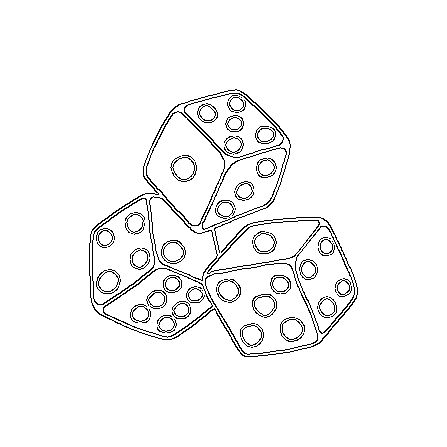
\includegraphics[width=0.6\linewidth]{figs/cover.png}
        \end{figure}
        \vfill
        
        {\large \textbf{Yifeng Xu}\\Institute of Computing Technology, CAS\\University of Chinese Academy of Sciences}\\[0.5cm]
    \end{center}
\end{titlepage}

\thispagestyle{empty}
\newpage


\nocite{*}
\section*{前言}

这是《概率导论》\cite{bertsekas2008introduction} 一书的笔记，主要包括初等概率论基础、极限理论、统计推断等内容，不包括原书第六章与第七章关于随机过程的内容。本笔记同时也参考了《统计推断》\cite{casella2009statistical} 的前四章。

《概率导论》原书将离散随机变量和连续随机变量分别写在第二章和第三章中，导致许多概念需要重复书写，因此本笔记将这两章合并为了一章。

本笔记附录 \ref{sec:random-variables} 整理总结了常用随机变量及其期望、方差、矩母函数及性质，附录 \ref{sec:two-normal} 整理了二元正态分布相关内容，附录~\ref{sec:normal-derive} 整理了正态分布的三个导出分布相关内容。
 \newpage
\tableofcontents \newpage
\section{样本空间与概率}

\subsection{概率模型}

\begin{definition}[概率模型的基本构成]
概率模型由样本空间和概率律构成：
\begin{itemize}
    \item 样本空间 $\Omega$：一个试验的所有可能结果的集合。
    \item 概率律：为试验结果的集合 $A$（称为事件）确定一个非负数 $\Pb(A)$，称为事件 $A$ 的概率。概率律需要满足概率公理。
\end{itemize}
\begin{figure}[H]
    \centering
    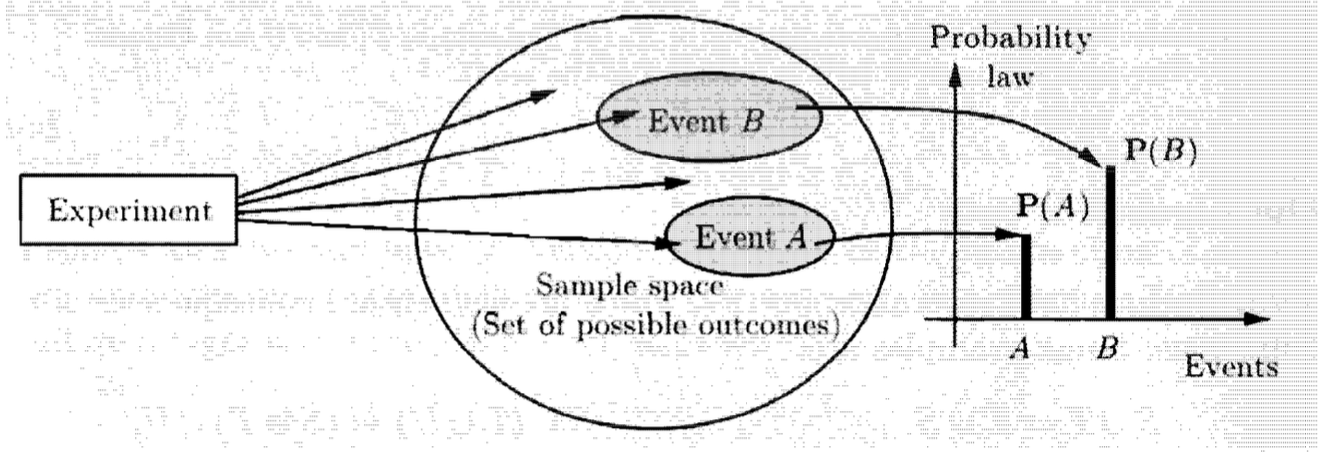
\includegraphics[width=0.8\linewidth]{figs/概率模型的基本构成.png}
    \caption{概率模型的基本构成}
    \label{fig:prob-model-components}
\end{figure}
\end{definition}

\begin{definition}[概率公理]
概率满足以下几条公理：
\begin{enumerate}
    \item 非负性：对一切事件 $A$，满足 $\Pb(A)\geq 0$.
    \item 归一化：整个样本空间为必然事件，即 $\Pb(\Omega)=1$.
    \item 可数可加性：设 $A_1,A_2,\ldots$ 是一列互不相容事件，则 $\Pb(A_1\cup A_2\cup\cdots)=\Pb(A_1)+\Pb(A_2)+\cdots$.
\end{enumerate}
\end{definition}

\begin{property}
设 $A,B,C$ 为事件，则由概率公理可以推导出如下性质：
\begin{itemize}
    \item 空事件概率为 0，即 $\Pb(\varnothing)=0$
    \item $A\subset B\implies \Pb(A)\leq \Pb(B)$
    \item $\Pb(A\cup B)=\Pb(A)+\Pb(B)-\Pb(A\cap B)$
    \item $\Pb(A\cup B)\leq \Pb(A)+\Pb(B)$
    \item $\Pb(A\cup B\cup C)=\Pb(A)+\Pb(A^c\cap B)+\Pb(A^c\cap B^c\cap C)$
\end{itemize}
\end{property}


\subsection{条件概率}

\begin{definition}[条件概率]
设 $A,B$ 为两个事件且 $\Pb(B)>0$，定义 $B$ 发生的条件下 $A$ 发生的概率为：\[\Pb (A\vert B)=\frac{\Pb(A\cap B)}{\Pb(B)},\quad \Pb(B)>0\]
\end{definition}

\begin{theorem}
条件概率是一个公理化定义下的概率，从而概率的所有性质都适用于条件概率。
\end{theorem}
\begin{proof}
只需验证条件概率是否满足非负性、归一化和可数可加性即可。
\begin{enumerate}
    \item 非负性：显然；
    \item 归一化：\[\Pb(\Omega\vert B)=\frac{\Pb(\Omega\cap B)}{\Pb(B)}=\frac{\Pb(B)}{\Pb(B)}=1\]
    \item 可数可加性：
    \begin{align*}
    \Pb\left(\left.\bigcup_{i=1}^nA_i\right\vert B\right)&=\frac{\Pb\left(\left(\bigcup_{i=1}^nA_i\right)\cap B\right)}{\Pb(B)}=\frac{\Pb\left(\bigcup_{i=1}^n(A_i\cap B)\right)}{\Pb(B)}\\
    &=\frac{\sum_{i=1}^n\Pb(A_i\cap B)}{\Pb(B)}=\sum_{i=1}^n\Pb(A_i\vert B)
    \end{align*}
\end{enumerate}
\end{proof}

\begin{theorem}[乘法公式]
设 $A,B$ 为两个事件，则由定义易知：\[\Pb (A\cap B)=\Pb(B)\Pb(A\vert B)\]
\end{theorem}

\begin{corollary}
设 $A_1,A_2,\ldots,A_n$ 为 $n$ 个事件，则：\[\Pb(A_1A_2\cdots A_n)=\Pb(A_1)\Pb(A_2\vert A_1)\Pb(A_3\vert A_1A_2)\cdots\Pb(A_n\vert A_1A_2\cdots A_{n-1})\]
\end{corollary}


\subsection{全概率公式和贝叶斯公式}

\begin{theorem}[全概率公式]
设 $A_1,A_2,\cdots,A_n$ 互不相容，$B\subset A_1\cup A_2\cup\cdots\cup A_n$，则：\[\Pb(B)=\sum_{i=1}^n\Pb(A_i)\Pb(B\vert A_i)\]
\end{theorem}
\begin{proof}
\[\Pb(B)=\Pb\left(B\cap \left(\bigcup_{i=1}^nA_i\right)\right)=\Pb\left(\bigcup_{i=1}^n(A_i\cap B)\right)=\sum_{i=1}^n\Pb(A_i\cap B)=\sum_{i=1}^n\Pb(A_i)\Pb(B\vert A_i)\]
\end{proof}

\begin{theorem}[贝叶斯公式]
设 $A_1,A_2,\cdots,A_n$ 互不相容且 $\Pb(A_i)>0$，$B\subset A_1\cup A_2\cup\cdots\cup A_n$，则：
\[\Pb(A_i\vert B)=\frac{\Pb(A_i\cap B)}{\Pb(B)}=\frac{\Pb(A_i)\Pb(B\vert A_i)}{\sum\limits_{j=1}^n\Pb(A_j)\Pb(B\vert A_j)}\]
其中 $\Pb(A_i)$ 称作先验概率，$\Pb(A_i\vert B)$ 称作后验概率。
\end{theorem}

\begin{remark}[关于贝叶斯公式的理解]
视事件 $A_i$ 是导致事件 $B$ 发生的原因，我们对于事件 $A_i$ 已有一个先验概率 $\Pb(A_i)$，现在事件 $B$ 发生了，这必然给我们带了一定的信息，于是我们可以由此修正 $A_i$ 发生的概率，得到 $\Pb(A_i\vert B)$，即后验概率。
\end{remark}


\subsection{独立性}

\begin{definition}[独立]
设 $A,B$ 是两个事件，称 $A$ 与 $B$ 独立，若：\[\Pb(A\cap B)=\Pb(A)\Pb(B)\]
\end{definition}
\begin{com}
若 $\Pb(B)\neq 0$，则 $A$ 与 $B$ 独立等价于：
\[\Pb(A\vert B)=\Pb(A)\]
直观上，这说明事件 $B$ 的发生与否并不给 $A$ 带来信息，不改变 $A$ 发生的概率。
\end{com}
\begin{note}
事件的独立性常常不能直观地看出来。例如，若事件 $A$ 与事件 $B$ 互不相容，并且 $\Pb(A)>0,\,\Pb(B)>0$，则它们一定不独立，因为 $\Pb(A\cap B)=0\neq\Pb(A)\Pb(B)$. 直观上，事件 $B$ 发生意味着 $A$ 一定没有发生，因此 $B$ 的发生与否会给 $A$ 带来信息。
\end{note}

\begin{theorem}
设事件 $A$ 与事件 $B$ 独立，则 $A$ 与 $B^c$ 也独立。
\end{theorem}
\begin{proof}
由于 $A$ 可写作两个不相容事件之并 $A=(A\cap B)\cup (A\cap B^c)$，故：
\[
\Pb(A)=\Pb(A\cap B)+\Pb(A\cap B^c)
\]
于是：
\[
\Pb(A\cap B^c)=\Pb(A)-\Pb(A\cap B)=\Pb(A)-\Pb(A)\Pb(B)=\Pb(A)(1-\Pb(B))=\Pb(A)\Pb(B^c)
\]
\end{proof}

\begin{definition}[条件独立]
给定事件 $C$，称事件 $A,B$ 在给定 $C$ 下条件独立，若：
\[\Pb(A\cap B\vert C)=\Pb(A\vert C)\Pb(B\vert C)\]
\end{definition}
\begin{com}
$A,B$ 条件独立并不能推出 $A,B$ 独立，反之亦不成立。
\end{com}

\begin{definition}[一组事件的相互独立性]
设 $A_1,A_2,\ldots,A_n$ 是一组事件，称它们相互独立，若：
\[
\Pb\left(\bigcap_{i\in S}A_i\right)=\prod_{i\in S}\Pb(A_i),\quad\forall S\subset\{1,2,\ldots,n\}
\]
\end{definition}
\begin{note}[两两独立与相互独立]
设 $A_1,A_2,A_3$ 相互独立，则有：
\begin{gather*}
\Pb(A_1\cap A_2)=\Pb(A_1)\Pb(A_2)\\
\Pb(A_2\cap A_3)=\Pb(A_1)\Pb(A_3)\\
\Pb(A_1\cap A_3)=\Pb(A_1)\Pb(A_3)\\
\Pb(A_1\cap A_2\cap A_3)=\Pb(A_1)\Pb(A_2)\Pb(A_3)
\end{gather*}
前三个式子称作两两独立。但是第四个式子也非常重要，它并不是前三个式子的推论；反之，第四个式子也不能推出前三个式子。
\end{note}
\begin{example}[两两独立不能推出独立]
设试验是抛掷两枚均匀的硬币，考虑事件：
\[H_1=\{\text{第一次正面}\},\quad H_2=\{\text{第二次正面}\},\quad D=\{\text{两次结果不同}\}\]
则易知 $H_1$ 与 $H_2$ 独立。另外，
\[
\Pb(D\vert H_1)=\frac{\Pb(D\cap H_1)}{\Pb(H_1)}=\frac{1/4}{1/2}=\frac{1}{2}=\Pb(D)
\]
故 $D$ 与 $H_1$ 独立。同理可知 $D$ 与 $H_2$ 独立，故 $H_1,H_2,D$ 两两独立。但是：
\[
\Pb(H_1\cap H_2\cap D)=0\neq \Pb(H_1)\Pb(H_2)\Pb(D)=\frac{1}{2}\cdot\frac{1}{2}\cdot\frac{1}{2}
\]
故 $H_1,H_2,D$ 不是独立的。
\end{example}
 \newpage
\section{随机变量}

\subsection{基本概念}

\begin{definition}[随机变量]
随机变量是试验结果的实值函数。
\begin{figure}[H]
    \centering
    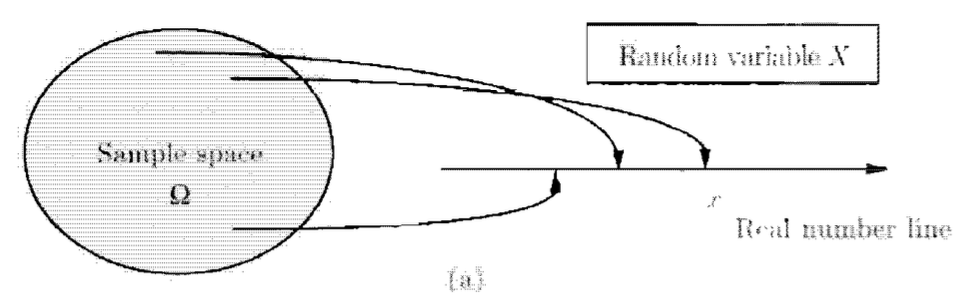
\includegraphics[width=0.65\linewidth]{figs/随机变量示意图.png}
    \caption{随机变量示意图}
    \label{fig:random-variable}
\end{figure}
\end{definition}
\begin{com}
一般用大写字母表示随机变量，小写字母表示其取值。
\end{com}

\begin{definition}[离散随机变量]
若一个随机变量的值域为有限集或可数集，则称这个随机变量是离散的。
\end{definition}

\begin{definition}[概率质量函数]
定义随机变量 $X$ 取值为 $x$ 的概率为事件 $\{X=x\}$ 的概率，即所有与 $x$ 对应的试验结果组成的事件的概率，记作 $p_X(x)$，即：
\[p_X(x)=\Pb(\{X=x\})\]
称 $p_X$ 为 $X$ 的概率质量函数 (PMF).
\end{definition}

\begin{property}
PMF 满足非负性和归一化条件：
\[\sum_x p_X(x)=\sum_x\Pb(X=x)=1\]
\end{property}
\begin{property}
设 $S$ 为任一 $X$ 可能取值的集合，则：
\[\Pb(X\in S)=\sum_{x\in S}p_X(x)\]
\end{property}

\begin{example}
常见的离散随机变量包括伯努利、二项、几何和泊松随机变量等，详见附录 \ref{sec:random-variables}.
\end{example}

\begin{definition}[连续随机变量，概率密度函数]
对随机变量 $X$，若存在一个非负函数 $f_X$，使得：
\[
\Pb(X\in B)=\int_Bf_X(x)\mathrm dx
\]
对实数轴的集合 $B$ 都成立\footnote{本书只考虑黎曼积分，且 $f_X$ 为有有限/可数个间断点的分段连续函数。}，则称 $X$ 为连续的随机变量，函数 $f_X$ 称为概率密度函数 (PDF). 特别地，当 $B$ 是一个区间时，有：
\[
\Pb(a\leq X\leq b)=\int_a^bf_X(x)\mathrm dx
\]
\end{definition}
\begin{property}
PDF 满足非负性和归一化条件：
\[\int_{-\infty}^{\infty}f_X(x)\mathrm dx=\Pb(-\infty<X<\infty)=1\]
\end{property}
\begin{property}
对于充分小的 $\delta$，有：
\[\Pb(x\leq X\leq x+\delta)=\int_x^{x+\delta}f_X(x)\mathrm dx\approx f(x)\cdot\delta\]
\end{property}

\begin{example}
常见的连续随机变量包括均匀、指数、柯西、伽马和正态随机变量等，详见附录 \ref{sec:random-variables}.
\end{example}


\subsection{分布函数}

\begin{definition}[分布函数]
设 $X$ 是一个随机变量（离散或连续），定义其分布函数（CDF）$F_X$ 为：
\[
F_X(x)=\Pb(X\leq x)=\begin{dcases}
    \sum_{k\leq x}p_X(k),&\text{$X$ 离散}\\
    \int_{-\infty}^xf_X(t)\mathrm dt,&\text{$X$ 连续}
\end{dcases}
\]
\end{definition}
\begin{com}
分布函数统一刻画了离散和连续情形。离散情形下的 PMF、连续情形下的 PDF 和一般情形下的 CDF 都是相应随机变量的概率律。
\end{com}

\begin{property}
设 $F_X$ 是随机变量 $X$ 的分布函数，则：
\begin{itemize}
    \item $F_X$ 单调非减。
    \item $F_X(x)\to 0\;(x\to-\infty),;F_X(x)\to1(x\to\infty)$.
    \item 当 $X$ 是离散随机变量时，$F_X$ 是阶梯函数。
    \item 当 $X$ 是连续随机变量时，$F_X$ 是连续函数。
\end{itemize}
\end{property}

\begin{theorem}[分布列与分布函数]
设 $X$ 是离散随机变量且取整数值，则：
\[
F_X(k)=\sum_{i=-\infty}^kp_X(i),\quad p_X(k)=F_X(k)-F_X(k-1)
\]
\end{theorem}
\begin{theorem}[概率密度函数与分布函数]
设 $X$ 是连续随机变量，则：
\[
F_X(x)=\int_{-\infty}^xf_X(t)\mathrm dt,\quad f_X(x)=\frac{\mathrm d}{\mathrm dx}F_X(x)
\]
第二个等式只在分布函数可微处成立。
\end{theorem}


\subsection{期望和方差}

\begin{definition}[期望/均值]
随机变量 $X$ 的期望定义为：
\[
\E X=\begin{dcases}
    \sum_x xp_X(x),&\text{$X$ 离散}\\
    \int_{-\infty}^{\infty}xf_X(x)\mathrm dx,&\text{$X$ 连续}
\end{dcases}
\]
特别地，对于连续情形，若 $f_X$ 不是绝对可积的，即 $\int_{-\infty}^\infty |x|f_X(x)\mathrm dx=\infty$，则称期望不存在。
\end{definition}

\begin{example}[柯西随机变量的期望不存在]
\TODO{}
\end{example}

\begin{definition}[矩，中心矩]
定义随机变量 $X$ 的 $n$ 阶矩为 $\E[X^n]$，$n$ 阶中心矩为 $\E[(X-\E X)^n]$.
\end{definition}

\begin{definition}[方差，标准差]
定义随机变量 $X$ 的方差为其 2 阶中心矩，标准差为方差的平方根：
\[
\var(X)=\E\left[(X-\E X)^2\right],\quad \sigma(X)=\sqrt{\var(X)}
\]
\end{definition}

\begin{theorem}[随机变量函数的期望]
设 $X$ 是一随机变量，则 $Y=g(X)$ 的期望为：
\[\E Y=\E[g(X)]=\begin{dcases}
    \sum_xg(x)p_X(x),&\text{$X$ 离散}\\
    \int_{-\infty}^{+\infty}g(x)f_X(x)\mathrm dx,&\text{$X$ 连续}
\end{dcases}
\]
因此，我们不必先求出 $Y$ 的分布，只需知道 $X$ 的分布就能求出 $Y$ 的期望。
\end{theorem}

\begin{theorem}[随机变量的线性函数的期望和方差]
设 $X$ 是一个随机变量，$Y=aX+b$，其中 $a,b$ 为常数，则：
\[\E Y=a\E X+b,\quad \var(Y)=a^2\var(X)\]
\end{theorem}
\begin{proof}
仅对离散情形证明，连续情形类似。
\begin{gather*}
\E Y=\sum_x(ax+b)p_X(x)=a\sum_x xp_X(x)+b\sum_xp_X(x)=a\E X+b\\
\var(Y)=\E[(Y-\E Y)^2]=\E[((aX+b)-(a\E X+b))^2]=a^2\E[(X-\E X)^2]=a^2\var(X)
\end{gather*}
\end{proof}

\begin{theorem}[用矩表达方差]
设 $X$ 是一个随机变量，则：
\[
\var(X)=\E[X^2]-(\E X)^2
\]
\end{theorem}
\begin{proof}
\begin{align*}
\var(X)&=\E\left[(X-\E X)^2\right]\\
&=\E\left[X^2-2X\E X+(\E X)^2\right]\\
&=\E[X^2]-2 \E X\cdot \E X+(\E X)^2\\
&=\E[X^2]-(\E X)^2
\end{align*}
\end{proof}

\begin{example}
常见随机变量的期望和方差及其推导过程见附录 \ref{sec:random-variables}.
\end{example}


\subsection{联合分布与边缘分布}

\begin{figure}[H]
    \centering
    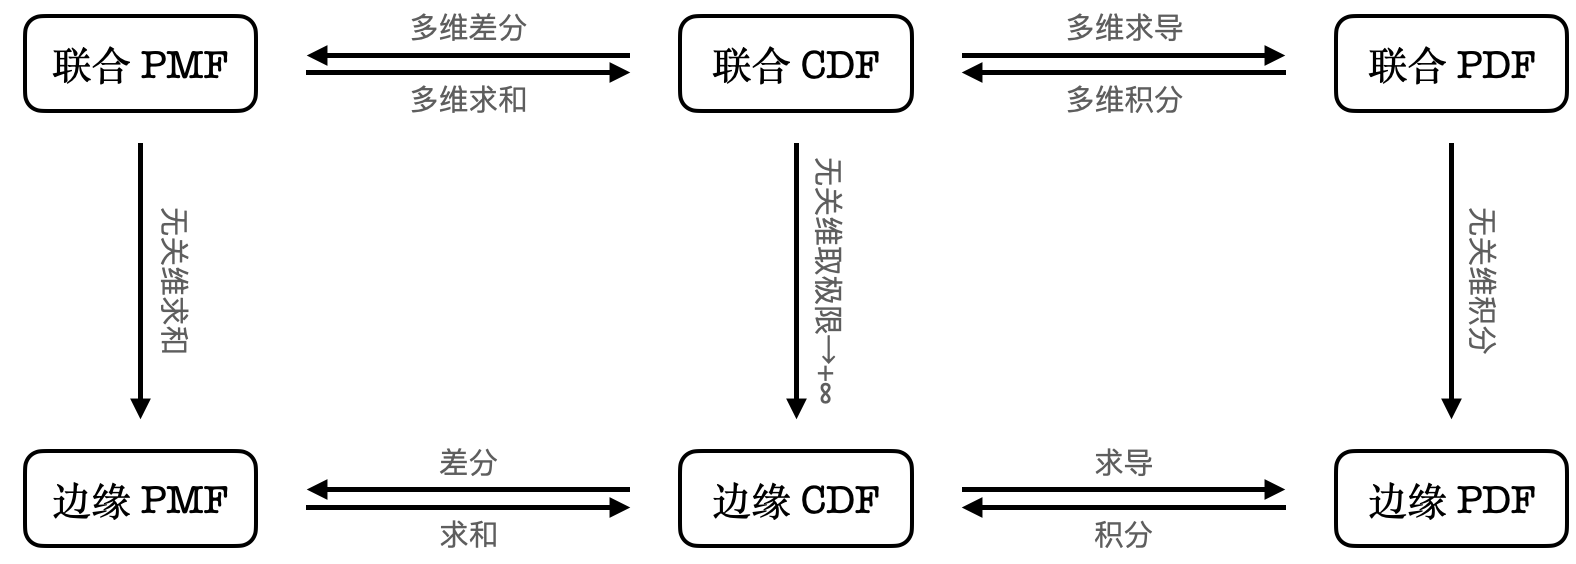
\includegraphics[width=0.8\linewidth]{figs/联合分布与边缘分布.png}
    \caption{联合分布与边缘分布的关系概览}
    \label{fig:union-marginal}
\end{figure}

\begin{definition}[联合概率质量函数]
设 $X,Y$ 是离散随机变量，定义 $(X,Y)$ 取值 $(x,y)$ 的概率为事件 $\{X=x,Y=y\}$ 的概率，记作 $p_{X,Y}(x,y)$，即：\[p_{X,Y}(x,y)=\Pb(X=x,Y=y)\]
称 $p_{X,Y}$ 为 $X,Y$ 的联合概率质量函数。
\end{definition}

\begin{definition}[联合概率密度函数]
设 $X,Y$ 是连续随机变量，若存在一个非负二元函数 $f_{X,Y}$ 使得：
\[
\Pb((X,Y)\in B)=\iint_{(x,y)\in B}f_{X,Y}(x,y)\mathrm dx\mathrm dy
\]
对平面上任意集合 $B$ 成立，则称 $f_{X,Y}$ 为联合概率密度函数。特别地，当 $B$ 是一个矩形区域时有：
\[
\Pb(a\leq X\leq b,c\leq Y\leq d)=\int_c^d\int_a^b f_{X,Y}(x,y)\mathrm dx\mathrm dy
\]
\end{definition}

\begin{property}
联合 PDF 满足归一化条件：
\[\int_{-\infty}^{\infty}\int_{-\infty}^{\infty}f_{X,Y}(x,y)\mathrm dx\mathrm dy=1\]
\end{property}
\begin{property}
对于充分小的 $\delta$，有：
\[\Pb(a\leq X\leq a+\delta,c\leq Y\leq c+\delta)=\int_c^{c+\delta}\int_a^{a+\delta}f_{X,Y}(x,y)\mathrm dx\mathrm dy\approx f_{X,Y}(a,c)\cdot\delta^2\]
\end{property}

\begin{theorem}[边缘概率质量函数]
设 $X,Y$ 是离散随机变量且联合 PMF 为 $p_{X,Y}$，则：
\[
p_X(x)=\sum_y p_{X,Y}(x,y),\quad p_Y(y)=\sum_xp_{X,Y}(x)
\]
称 $p_X$ 和 $p_Y$ 为边缘概率质量函数。
\end{theorem}

\begin{theorem}[边缘概率密度函数]
设 $X,Y$ 是连续随机变量且联合 PDF 为 $f_{X,Y}$，则：
\[
f_X(x)=\int_{-\infty}^{\infty}f_{X,Y}(x,y)\mathrm dy,\quad f_Y(y)=\int_{-\infty}^{\infty}p_{X,Y}(x)\mathrm dx
\]
称 $f_X$ 和 $f_Y$ 为边缘概率密度函数。
\end{theorem}

\begin{definition}[联合分布函数]
设 $X,Y$ 是两个随机变量（离散或连续），定义其联合分布函数为：
\[
F_{X,Y}(x,y)=\Pb(X\leq x,Y\leq y)
\]
\end{definition}

\begin{theorem}[联合概率密度函数与联合分布函数]
若随机变量 $X,Y$ 有联合概率密度函数 $f_{X,Y}$，则：
\[
F_{X,Y}(x,y)=\int_{-\infty}^x\int_{-\infty}^yf_{X,Y}(s,t)\mathrm ds\mathrm dt,\quad f_{X,Y}(x,y)=\frac{\partial^2}{\partial x\partial y}F_{X,Y}(x,y)
\]
\end{theorem}

\begin{theorem}[随机变量的二元函数的期望]
设 $X$ 和 $Y$ 是随机变量，则 $Z=g(X,Y)$ 的期望为：
\[
\E Z=\E[g(X,Y)]=\begin{dcases}
    \sum_{x}\sum_{y}g(x,y)p_{X,Y}(x,y),&\text{$X,Y$ 离散}\\
    \int_{-\infty}^{\infty}\int_{-\infty}^{\infty}g(x,y)f_{X,Y}(x,y)\mathrm dx\mathrm dy,&\text{$X,Y$ 连续}
\end{dcases}
\]
\end{theorem}

\begin{theorem}[随机变量的二元线性函数的期望]
设 $X$ 和 $Y$ 是随机变量，$a,b,c$ 为常数，则：
\[
\E[aX+bY+c]=a\E X+b\E Y+c
\]
\end{theorem}

\begin{theorem}[随机变量的多元线性函数的期望]
设 $X_1,X_2,\ldots,X_n$ 是 $n$ 个随机变量，$a_1,a_2,\ldots,a_n$ 是 $n$ 个常数，则：
\[
\E[a_1X_1+a_2X_2+\cdots+a_nX_n]=a_1\E X_2+a_2\E X_2+\cdots+a_n\E X_n
\]
\end{theorem}


\subsection{条件}

\begin{definition}[条件分布]
设 $X,Y$ 是离散随机变量，定义给定 $Y=y$ 下 $X$ 的条件概率质量函数为：
\[
p_{X\vert Y}(x\vert y)=\Pb(X=x\vert Y=y)=\frac{\Pb(X=x,Y=y)}{\Pb(Y=y)}=\frac{p_{X,Y}(x,y)}{p_Y(y)}
\]
类似地，设 $X,Y$ 是连续随机变量，定义给定 $Y=y$ 下 $X$ 的条件概率密度函数为：
\[
f_{X\vert Y}(x\vert y)=\frac{f_{X,Y}(x,y)}{f_Y(y)}
\]
\end{definition}

\begin{property}
条件 PMF/PDF 满足归一化条件：
\begin{gather*}
\sum_x p_{X\vert Y}(x\vert y)=1,\quad\text{$X$ 离散}\\
\int_{-\infty}^{\infty}f_{X\vert Y}(x\vert y)\mathrm dx=1,\quad\text{$X$ 连续}
\end{gather*}
\end{property}

\begin{theorem}[条件分布与联合分布]
设 $X,Y$ 是随机变量，由定义可知：
\begin{gather*}
p_{X,Y}(x,y)=p_Y(y)p_{X\vert Y}(x\vert y)=p_X(x)p_{Y\vert X}(y\vert x),\quad\text{$X$ 离散}\\
f_{X,Y}(x,y)=f_Y(y)f_{X\vert Y}(x\vert y)=f_X(x)f_{Y\vert X}(y\vert x),\quad\text{$X$ 连续}
\end{gather*}
\end{theorem}

\begin{theorem}[条件分布与边缘分布]
设 $X,Y$ 是随机变量，则根据全概率公式，有：
\begin{gather*}
p_X(x)=\sum_y p_{X\vert Y}(x\vert y)p_Y(y),\quad\text{$X$ 离散}\\
f_X(x)=\int_{-\infty}^{\infty} f_{X\vert Y}(x\vert y)f_Y(y)\mathrm dy,\quad\text{$X$ 连续}
\end{gather*}
\end{theorem}

\begin{theorem}[贝叶斯公式]
设 $X,Y$ 是随机变量，则有：
\begin{gather*}
p_{X\vert Y}(x\vert y)=\frac{p_{X,Y}(x,y)}{p_Y(y)}=\frac{p_{Y\vert X}(y\vert x)p_X(x)}{\sum_x p_{Y\vert X}(y\vert x)p_X(x)},\quad\text{$X,Y$ 离散}\\
f_{X\vert Y}(x\vert y)=\frac{f_{X,Y}(x,y)}{f_Y(y)}=\frac{f_{Y\vert X}(y\vert x)f_X(x)}{\int_{-\infty}^{\infty}f_{Y\vert X}(y\vert x)f_X(x)\mathrm dx},\quad\text{$X,Y$ 连续}
\end{gather*}
\end{theorem}

\begin{definition}[条件期望]
设 $X,Y$ 是随机变量，则给定 $Y=y$ 下 $X$ 的条件期望为：
\[
\E[X\vert Y=y]=\begin{dcases}
    \sum_xxp_{X\vert Y}(x\vert y),&\text{$X$ 离散}\\
    \int_{-\infty}^{\infty}xf_{X\vert Y}(x\vert y)\mathrm dx,&\text{$X$ 连续}
\end{dcases}
\]
对于随机变量的函数 $g(X)$，有：
\[
\E[g(X)\vert Y=y]=\begin{dcases}
    \sum_xg(x)p_{X\vert Y}(x\vert y),&\text{$X$ 离散}\\
    \int_{-\infty}^{\infty}g(x)f_{X\vert Y}(x\vert y)\mathrm dx,&\text{$X$ 连续}
\end{dcases}
\]
\end{definition}

\begin{note}
$\E[X|Y=y]$ 是一个数，其值依赖于 $y$，因此 $\E[X|Y]$ 是关于随机变量 $Y$ 的函数，从而也是一个随机变量。
\end{note}

\begin{theorem}[全期望公式]
设 $X,Y$ 是随机变量（离散或连续）且 $X$ 期望存在，则：
\[
\E X=\E[\E[X\vert Y]]=\begin{dcases}
    \sum_y \E[X\vert Y=y]p_Y(y),&\text{$Y$ 离散}\\
    \int_{-\infty}^{\infty} \E[X\vert Y=y]f_Y(y)\mathrm dy,&\text{$Y$ 连续}
\end{dcases}
\]
\end{theorem}
\begin{proof}
仅对离散情形证明，连续情形类似。
\begin{align*}
\E X&=\sum_x xp_X(x)\\
&=\sum_x x\sum_yp_{X|Y}(x\vert y)p_Y(y)\\
&=\sum_yp_Y(y)\sum_xxp_{X|Y}(x\vert y)\\
&=\sum_y \E[X\vert Y=y]p_Y(y)
\end{align*}
其中第二行应用了全概率公式。
\end{proof}

\begin{remark}
全期望公式常常是“反过来”使用的：当 $\mathbb EX$ 不好计算时，引入 $Y$ 转而计算 $\mathbb E[\mathbb E[X\vert Y]]$.
\end{remark}

\begin{definition}[条件方差]
设 $X,Y$ 是随机变量，则给定 $Y=y$ 下 $X$ 的条件方差为：
\[
\var(X\vert Y=y)=\E[(X-\E[X\vert Y=y])^2\vert Y=y]
\]
\end{definition}

\begin{note}
$\var(X\vert Y=y)$ 是一个数，其值依赖于 $y$，因此 $\var(X\vert Y)$ 是关于随机变量 $Y$ 的函数，从而也是一个随机变量，并且有：
\[
\var(X\vert Y)=\E[(X-\E[X\vert Y])^2\vert Y]=\E[X^2\vert Y]-(\E[X\vert Y])^2
\]
\end{note}

\begin{theorem}[全方差公式]
设 $X,Y$ 是随机变量且 $X$ 方差存在，则：
\[
\var(X)=\E[\var(X\vert Y)]+\var(\E[X\vert Y])
\]
\end{theorem}
\begin{proof}
\begin{align*}
\var(X)&=\E[X^2]-(\E X)^2\\
&=\E[\E[X^2\vert Y]]-(\E[\E[X\vert Y]])^2\\
&=\E[\E[X^2\vert Y]]-\E[(\E[X\vert Y])^2]+\E[(\E[X\vert Y])^2]-(\E[\E[X\vert Y]])^2\\
&=\E[\var(X\vert Y)]+\var(\E[X\vert Y])
\end{align*}
\end{proof}


\subsection{独立性}

\begin{definition}[独立]
设 $X,Y$ 是随机变量，称 $X$ 与 $Y$ 独立，若：
\begin{gather*}
p_{X,Y}(x,y)=p_X(x)p_Y(y),\quad\forall x,y,\quad\text{$X,Y$ 离散}\\
f_{X,Y}(x,y)=f_X(x)f_Y(y),\quad\forall x,y,\quad\text{$X,Y$ 连续}
\end{gather*}
\end{definition}
\begin{com}
离散情形下，若 $p_Y(y)>0$，则 $X$ 与 $Y$ 独立等价于：
\[p_{X\vert Y}(x\vert y)=p_X(x),\;\forall y\]
直观上，这说明 $Y$ 的取值不会给 $X$ 的取值带来信息。连续情形同理。
\end{com}

\begin{definition}[条件独立]
设 $X,Y,Z$ 是随机变量，给定 $Z=z$ 下（设 $p_Z(z)>0$ 或 $f_Z(z)>0$），称随机变量 $X$ 与 $Y$ 条件独立，若：
\begin{gather*}
p_{X,Y\vert Z}(x,y\vert z)=p_{X\vert Z}(x\vert z)p_{Y\vert Z}(y\vert z),\quad\forall x,y,\quad\text{$X,Y$ 离散}\\
f_{X,Y\vert Z}(x,y\vert z)=f_{X\vert Z}(x\vert z)f_{Y\vert Z}(y\vert z),\quad\forall x,y,\quad\text{$X,Y$ 连续}
\end{gather*}
\end{definition}

\begin{theorem}
若随机变量 $X,Y$ 相互独立，则：
\[
\E[XY]=\E X\E Y
\]
进一步地，对任意函数 $g,h$，有：
\[
\E[g(X)h(Y)]=\E[g(X)]\E[h(Y)]
\]
\end{theorem}
\begin{proof}
仅对离散情形证明，连续情形类似。
\begin{align*}
\E[XY]&=\sum_x\sum_y xyp_{X,Y}(x,y)\\
&=\sum_x\sum_y xyp_X(x)p_Y(y)\\
&=\sum_x xp_X(x)\sum_y yp_Y(y)\\
&=\E X\E Y
\end{align*}
第二个式子类似可证。
\end{proof}

\begin{corollary}
若随机变量 $X,Y$ 独立，则对任意函数 $g,h$，有 $g(X)$ 与 $h(Y)$ 独立。
\end{corollary}

\begin{theorem}
若随机变量 $X,Y$ 相互独立，则：
\[
\var(X+Y)=\var(X)+\var(Y)
\]
\end{theorem}
\begin{proof}
令 $\tilde X=X-\E X,\,\tilde Y=Y-\E Y$，由于方差在加减常数后保持不变，所以：
\begin{align*}
\var(X+Y)&=\var(\tilde X+\tilde Y)\\
&=\E[(\tilde X+\tilde Y)^2]\\
&=\E[{\tilde X}^2+2\tilde X\tilde Y+{\tilde Y}^2]\\
&=\E[{\tilde X}^2]+2\E[\tilde X\tilde Y]+\E[{\tilde Y}^2]\\
&=\var X+\var Y
\end{align*}
其中利用了 $\E[\tilde X\tilde Y]=\E[\tilde X]\E[\tilde Y]=0$.
\end{proof}

\begin{definition}[多个随机变量独立性]
称随机变量 $X,Y,Z$ 相互独立，若：
\begin{gather*}
p_{X,Y,Z}(x,y,z)=p_X(x)p_Y(y)p_Z(z),\quad\forall x,y,z,\quad\text{$X,Y,Z$ 离散}\\
f_{X,Y,Z}(x,y,z)=f_X(x)f_Y(y)f_Z(z),\quad\forall x,y,z,\quad\text{$X,Y,Z$ 连续}
\end{gather*}
\end{definition}

\begin{theorem}[多个独立随机变量和的方差]
设 $X_1,X_2,\ldots,X_n$ 为相互独立的随机变量，则：
\[
\var(X_1+X_2+\cdots+X_n)=\var(X_1)+\var(X_2)+\cdots+\var(X_n)
\]
\end{theorem}


% \subsection{正态随机变量}

% \begin{definition}[正态随机变量/高斯随机变量]
% 称连续随机变量 $X$ 为正态或高斯的，若其 PDF 为：
% \[
% f_X(x)=\frac{1}{\sqrt{2\pi}\sigma}e^{-\frac{(x-\mu)^2}{2\sigma^2}}
% \]
% 其中 $\mu,\sigma$ 是参数。
% \end{definition}

% \begin{theorem}[正态分布的均值和方差]
% 设 $X$ 为
% \end{theorem}
 \newpage
\section{随机变量的深入内容}

\subsection{随机变量的函数的分布}

\begin{theorem}[随机变量的函数]
设 $X$ 是离散随机变量，则 $Y=g(X)$ 的 PMF 为：
\[p_Y(y)=\sum_{\{x|y=g(x)\}}p_X(x)\]
设 $X$ 是连续随机变量，则 $Y=g(X)$ 的 CDF 为：
\[F_Y(y)=\Pb(Y\leqslant y)=\Pb(g(X)\leqslant y)=\int\limits_{\{x|g(x)\leqslant y\}}f_X(x)\mathrm dx\]
进而 PDF 为：
\[f_Y(y)=\frac{\mathrm d}{\mathrm dy}F_Y(y)\]
\end{theorem}

\begin{theorem}[线性函数情形]
\label{thm:rv-linear}
设 $X$ 是连续随机变量，$a,b\in\R$ 且 $a\neq0$，设 $Y=aX+b$，则：
\[f_Y(y)=\frac{1}{|a|}f_X\left(\frac{y-b}{a}\right)\]
\end{theorem}
\begin{proof}
先求 $Y$ 的 CDF：
\[F_Y(y)=\Pb(Y\leqslant y)=\Pb(aX+b\leqslant y)=\begin{cases}\Pb\left(X\leqslant \frac{y-b}{a}\right)=F_X\left(\frac{y-b}{a}\right),&a>0\\\Pb\left(X\geqslant \frac{y-b}{a}\right)=1-F_X\left(\frac{y-b}{a}\right),&a<0\end{cases}\]
然后求导得到 $Y$ 的 PDF：
\[f_Y(y)=\frac{\mathrm dF_Y(y)}{\mathrm dy}=\begin{cases}\frac{1}{a}f_X\left(\frac{y-b}{a}\right),&a>0\\-\frac{1}{a}f_X\left(\frac{y-b}{a}\right),&a<0\end{cases}\quad=\quad\frac{1}{|a|}f_X\left(\frac{y-b}{a}\right)\]
\end{proof}

\begin{example}[正态分布的线性变换仍然是正态分布]
设 $X\sim N(\mu,\sigma^2)$，$a,b\in\mathbb R$ 且 $a\neq0$，$Y=aX+b$，则根据定理 \ref{thm:rv-linear}，有：
\begin{align*}
f_{Y}(y)&=\frac{1}{|a|}f_X\left(\frac{y-b}{a}\right)\\
&=\frac{1}{\sqrt{2\pi}\sigma|a|}\exp\left({-\frac{\left(\frac{y-b}{a}-\mu\right)^2}{2\sigma^2}}\right)\\
&=\frac{1}{\sqrt{2\pi}\sigma|a|}\exp\left({-\frac{(y-a\mu-b)^2}{2a^2\sigma^2}}\right)
\end{align*}
所以，$Y=aX+b\sim N(a\sigma+b,a^2\sigma^2)$.
\end{example}

\begin{theorem}[单调函数情形]
设 $X$ 是连续随机变量，$g$ 是严格单调的可逆函数，且其反函数 $h$ 可微，则 $Y=g(X)$ 在其支撑集 $\{y\mid f_Y(y)>0\}$ 上的 PDF 是：
\[f_Y(y)=f_X(h(y))\left|\frac{\mathrm d}{\mathrm dy}h(y)\right|\]
\end{theorem}
\begin{proof}
先求 $Y$ 的 CDF：
\[F_Y(y)=\Pb(Y\leqslant y)=\begin{cases}\Pb(X\leqslant h(y))=F_X(h(y)),&g\;\text{单调递增}\\\Pb(X\geqslant h(y))=1-F_X(h(y)),&g\;\text{单调递减}\end{cases}\]
于是求导得：
\[f_Y(y)=\begin{cases}f_X(h(y))h'(y),&g\;\text{单调递增}\\-f_X(h(y))h'(y),&g\;\text{单调递减}\end{cases}\quad =\quad f_X(h(y))\left|\frac{\mathrm d}{\mathrm dy}h(y)\right|\]
\end{proof}

\begin{theorem}[随机变量的二元函数]
设 $X,Y$ 是离散随机变量，则 $Z=g(X,Y)$ 的 PMF 为：
\[p_Z(z)=\sum_{\{(x,y)|z=g(x,y)\}}p_{X,Y}(x,y)\]
设 $X,Y$ 是连续随机变量，则 $Z=g(X,Y)$ 的 CDF 为：
\[F_Z(z)=\Pb(Z\leqslant z)=\Pb(g(X,Y)\leqslant z)=\iint\limits_{\{(x,y)|g(x,y)\leqslant z\}}f_{X,Y}(x,y)\mathrm dx\mathrm dy\]
进而 PDF 为：
\[f_Z(z)=\frac{\mathrm d}{\mathrm dz}F_Z(z)\]
\end{theorem}

\begin{example}[瑞利分布]
设 $X,Y\sim N(0,\sigma^2)$ 且相互独立，$R=\sqrt{X^2+Y^2}$，称 $R$ 服从瑞利分布。
首先计算 CDF：
\begin{align*}
F_R(r)&=\Pb(R\leqslant r)=\Pb(X^2+Y^2\leqslant r^2)\\
&=\iint\limits_{\{(x,y)|x^2+y^2\leqslant r^2\}}p_{X,Y}(x,y)\mathrm dx\mathrm dy\\
&=\iint\limits_{x^2+y^2\leqslant r^2}\frac{1}{2\pi\sigma^2}e^{-\frac{x^2+y^2}{2\sigma^2}}\mathrm dx\mathrm dy\\
&=\frac{1}{2\pi\sigma^2}\int_0^{2\pi}\mathrm d\theta\int_0^{r}e^{-\frac{\rho^2}{2\sigma^2}}\rho\mathrm d\rho\\
&=\left.e^{-\frac{\rho^2}{2\sigma^2}}\right|_{r}^0=1-e^{-\frac{r^2}{2\sigma^2}}
\end{align*}
故瑞利分布的 PDF 为：
\[f_R(r)=\frac{\mathrm dF_R(r)}{\mathrm dr}=\frac{r}{\sigma^2}e^{-\frac{r^2}{2\sigma^2}}\]
\end{example}

\begin{theorem}[极值分布]
设 $X,Y$ 是独立的随机变量，$M=\max(X,Y),N=\min(X,Y)$，则：
\[F_M(z)=F_X(z)F_Y(z),\qquad F_N(z)=1-(1-F_X(z))(1-F_Y(z))\]
\end{theorem}
\begin{proof}
\begin{align*}
F_M(z)&=\Pb(M\leqslant z)=\Pb(X\leqslant z, Y\leqslant z)=\Pb(X\leqslant z)\Pb(Y\leqslant z)=F_X(z)F_Y(z)\\
F_N(z)&=\Pb(N\leqslant z)=1-\Pb(N>z)=1-\Pb(X>z, Y>z)\\
&=1-\Pb(X>z)\Pb(Y>z)=1-(1-F_X(z))(1-F_Y(z))
\end{align*}
\end{proof}

\begin{corollary}
设 $X_1,X_2,\cdots,X_n$ 是 $n$ 个相互独立的随机变量，$M=\max\limits_{1\leqslant i\leqslant n}X_i$，$N=\min\limits_{1\leqslant i\leqslant n}X_i$，则：
\[F_M(z)=\prod_{i=1}^nF_{X_i}(z),\qquad F_N(z)=1-\prod_{i=1}^n(1-F_{X_i}(z))\]
\end{corollary}

\begin{theorem}[独立随机变量之和——卷积]
\label{thm:sum-ind-rv}
设 $X,Y$ 是独立的离散随机变量，$Z=X+Y$，则：
\[p_Z(z)=\sum_x p_X(x)p_Y(z-x)\]
设 $X,Y$ 是独立的连续随机变量，$Z=X+Y$，则：
\[f_Z(z)=\int_{-\infty}^{+\infty} f_X(x)f_Y(z-x)\mathrm dx\]
称上述两个式子为卷积（convolution）。
\end{theorem}

\begin{example}[独立正态随机变量之和仍服从正态分布]
设 $X\sim N(\mu_x,\sigma_x^2)$，$Y\sim N(\mu_y,\sigma_y^2)$ 且相互独立，$Z=X+Y$，则根据定理 \ref{thm:sum-ind-rv}，有：
\[
f_Z(z)=\int_{-\infty}^{+\infty}\frac{1}{2\pi\sigma_x\sigma_y}e^{-\frac{(x-\mu_x)^2}{2\sigma_x^2}-\frac{(z-x-\mu_y)^2}{2\sigma_y^2}}\mathrm dx=\int_{-\infty}^{+\infty}\frac{1}{2\pi\sigma_x\sigma_y}e^{-\frac{1}{2}\left[\frac{u^2}{\sigma_x^2}+\frac{(v-u)^2}{\sigma_y^2}\right]}\mathrm du
\]
其中做了代换 $u=x-\mu_x,\,v=z-\mu_x-\mu_y$. 由于：
\[
\frac{u^2}{\sigma_x^2}+\frac{(v-u)^2}{\sigma_y^2}=\frac{u^2}{\sigma_x^2}+\frac{u^2}{\sigma_y^2}+\frac{v^2}{\sigma_y^2}-\frac{2uv}{\sigma_y^2}=\left(\frac{\sqrt{\sigma_x^2+\sigma_y^2}}{\sigma_x\sigma_y}u-\frac{\sigma_x v}{\sigma_y\sqrt{\sigma_x^2+\sigma_y^2}}\right)^2+\frac{v^2}{\sigma_x^2+\sigma_y^2}
\]
令 $t=\frac{\sqrt{\sigma_x^2+\sigma_y^2}}{\sigma_x\sigma_y}u-\frac{\sigma_x v}{\sigma_y\sqrt{\sigma_x^2+\sigma_y^2}}$，则：
\[
f_Z(z)=\frac{1}{2\pi\sigma_x\sigma_y}\frac{\sigma_x\sigma_y}{\sqrt{\sigma_x^2+\sigma_y^2}}e^{\frac{v^2}{\sigma_x^2+\sigma_y^2}}\int_{-\infty}^{+\infty}e^{-\frac{1}{2}t^2}\mathrm dt=\frac{1}{\sqrt{2\pi}\sqrt{\sigma_x^2+\sigma_y^2}}e^{\frac{(z-\mu_x-\mu_y)^2}{\sigma_x^2+\sigma_y^2}}
\]
所以 $Z\sim N(\mu_x+\mu_y,\sigma_x^2+\sigma_y^2)$.
\end{example}

\begin{example}[$n$ 个独立正态随机变量之和]
\label{ex:ind-normal-sum}
设 $X_i\sim N(\mu_i,\sigma_i^2),\,i=1,2,\ldots,n$ 且相互独立，则：
\[\sum\limits_{i=1}^nX_i\sim N\left(\sum\limits_{i=1}^n\mu_i,\sum\limits_{i=1}^n\sigma_i^2\right)\]
\end{example}

\begin{example}[独立柯西随机变量之和仍服从柯西分布]
\TODO{}
\end{example}

\begin{theorem}[随机变量的多元函数（可逆函数情形）]
设 $\mathbf{X}=(X_1,X_2,\cdots,X_n)$ 是一个随机向量，$T$ 是 $\R ^n$ 上的一可逆映射，$\mathbf Y=T(\mathbf X)$，则 $\mathbf Y$ 的 PDF 为：
\[f_{\mathbf Y}(\mathbf y)=f_{\mathbf X}(T^{-1}(\mathbf y))|J|\]
其中，$J$ 表示 $T^{-1}:\mathbf y\mapsto \mathbf x$，即 $\mathbf x=T^{-1}(\mathbf y)$ 的雅各比行列式：
\[
J=\begin{vmatrix}
\dfrac{\partial x_1}{\partial y_1}&\dfrac{\partial x_1}{\partial y_2}&\cdots&\dfrac{\partial x_1}{\partial y_n}\\[3ex]
\dfrac{\partial x_2}{\partial y_1}&\dfrac{\partial x_2}{\partial y_2}&\cdots&\dfrac{\partial x_2}{\partial y_n}\\[2ex]
\vdots&\vdots&\vdots&\vdots\\[2ex]
\dfrac{\partial x_n}{\partial y_1}&\dfrac{\partial x_n}{\partial y_2}&\cdots&\dfrac{\partial x_n}{\partial y_n}\end{vmatrix}
\]
\end{theorem}
\begin{proof}
设 $D\subset \R^n$ 是一个性质好的集合，则：
\begin{align*}
\Pb(\mathbf Y\in D)&=\Pb(T(\mathbf X)\in D)\\
&=\Pb(\mathbf X\in T^{-1}(D))&\text{两边同时施以}\;T^{-1}\\
&=\int_{T^{-1}(D)}f_{\mathbf X}(\mathbf x)\mathrm d\mathbf x\\
&=\int_{D}f_{\mathbf X}(T^{-1}(y))|J|\mathrm d\mathbf y&\text{变量代换}\;\mathbf y=T(\mathbf x)
\end{align*}
又：
\[\Pb(\mathbf Y\in D)=\int_Df_\mathbf Y(\mathbf y)\mathrm d\mathbf y\]
根据 $D$ 一定的任意性，可知：
\[f_{\mathbf Y}(\mathbf y)=f_{\mathbf X}(T^{-1}(\mathbf y))|J|\]
\end{proof}


\subsection{协方差与相关系数}

\begin{figure}[H]
    \centering
    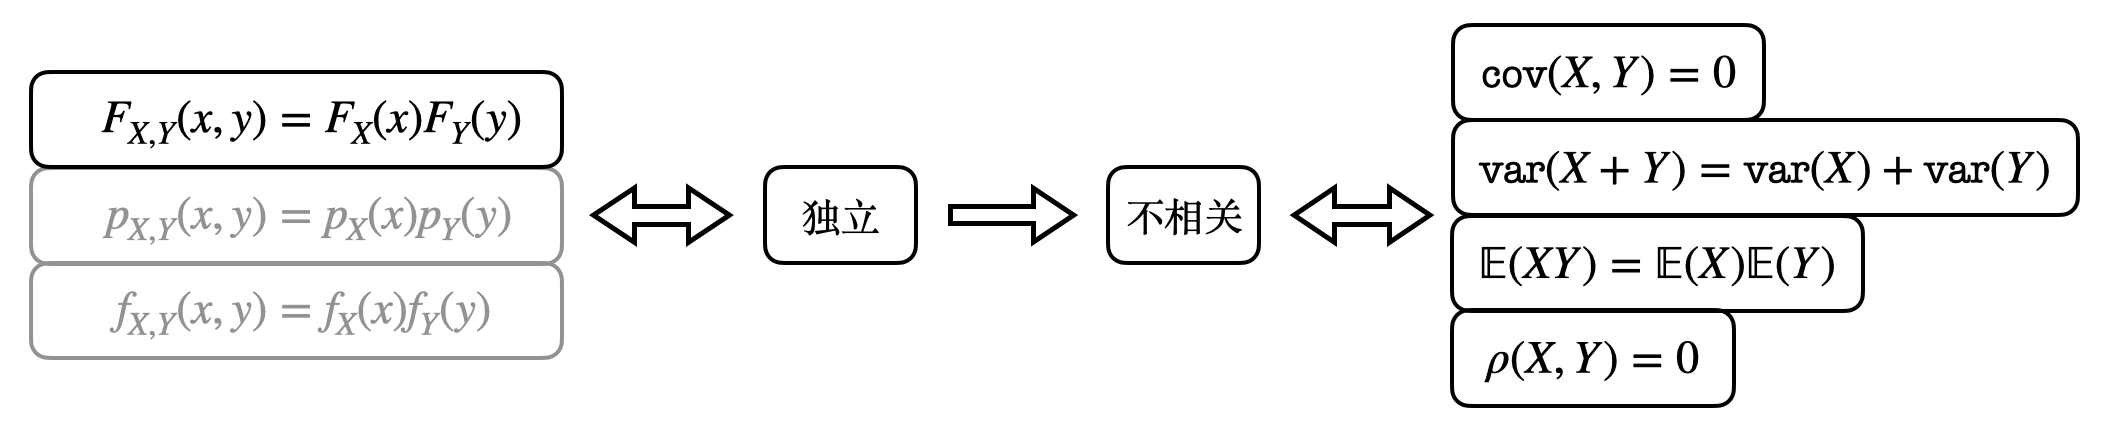
\includegraphics[width=0.9\linewidth]{figs/随机变量的独立性与相关性.png}
    \caption{随机变量的独立性与相关性示意图}
    \label{fig:independence-correlation}
\end{figure}

\begin{definition}[协方差与相关系数]
设 $X,Y$ 是两个随机变量，定义协方差与相关系数分别为：
\[
\cov(X,Y)=\E [(X-\E  X)(Y-\E  Y)],\quad\rho(X,Y)=\frac{\cov(X,Y)}{\sqrt{\var X\var Y}}
\]
当 $\cov(X,Y)=\rho(X,Y)=0$ 时，称 $X$ 和 $Y$ 不相关。
\end{definition}

\begin{property}
从定义出发容易证明以下性质：
\begin{itemize}
    \item $\cov(X,X)=\var(X)$
    \item $\cov(X,aY+b)=a\cdot\cov(X,Y)$ 
    \item $\cov(X,Y+Z)=\cov(X,Y)+\cov(X,Z)$
\end{itemize}
\end{property}

\begin{property}
$|\rho(X,Y)|\leq 1$.
\end{property}
\begin{proof}
对 $\forall t\in \R$，由于 $\var(Y-tX)=t^2\var X-2t\cov(X,Y)+\var Y\geq 0$，所以：
\[\Delta=4\cov^2(X,Y)-4\var X\var Y\leq 0\]
即有 $|\rho(X,Y)|\leq 1$.
\end{proof}

\begin{theorem}
设 $X,Y$ 是两个随机变量，则：
\[\cov(X,Y)=\E[XY]-\E X\E Y\]
\end{theorem}
\begin{proof}
\begin{align*}
\cov(X,Y)&=\E[(X-\E X)(Y-\E Y)]\\
&=\E[XY-\E X\cdot Y-X\cdot \E Y+\E X\E Y]\\
&=\E[XY]-\E X\cdot\E Y-\E X\cdot\E Y+\E X\cdot\E Y\\
&=\E[XY]-\E X\E Y
\end{align*}
\end{proof}

\begin{corollary}[独立与相关]
设 $X,Y$ 是两个随机变量，若 $X,Y$ 独立，则 $X,Y$ 不相关。
\end{corollary}
\begin{note}
反之不成立，不相关不能推出独立。
\end{note}

\begin{example}[不相关且不独立]
设随机变量 $X,Y$ 以 $1/4$ 的概率取 $(1,0),(0,1),(-1,0),(0,-1)$，则 $\E X=\E Y=\E[XY]=0$，于是 $\cov(X,Y)=\E[XY]-\E X\E Y=0$，故 $X,Y$ 不相关。但是 $p_{X,Y}(1,0)=1/4\neq p_X(1)p_Y(0)=1/4\cdot 1/2=1/8$，故二者不独立。直观上，$X$ 取非零值就要求 $Y$ 取零值，因此不独立。
\end{example}

\begin{theorem}[随机变量和的方差]
设随机变量 $X,Y$ 有有限的方差，则：
\[\var(X+Y)=\var X+2\cov(X,Y)+\var Y\]
更一般的，设随机变量 $X_1,X_2,\ldots,X_n$ 有有限的方差，则：
\[
\var\left(\sum_{i=1}^n X_i\right)=\sum_{i=1}^n\var(X_i)+\sum_{\{(i,j)\mid i\neq j\}}\cov(X_i,X_j)
\]
\end{theorem}
\begin{proof}
设 $\tilde X_i=X_i-\E[X_i]$，则：
\begin{align*}
\var\left(\sum_{i=1}^n X_i\right)&=\E\left[\left(\sum_{i=1}^n{\tilde X_i}^2\right)^2\right]\\
&=\E\left[\sum_{i=1}^n\sum_{j=1}^n\tilde X_i\tilde X_j\right]\\
&=\sum_{i=1}^n\sum_{j=1}^n\E\left[\tilde X_i\tilde X_j\right]\\
&=\sum_{i=1}^n\E[{\tilde X_i}^2]+\sum_{\{(i,j)\mid i\neq j\}}^n\E\left[\tilde X_i\tilde X_j\right]\\
&=\sum_{i=1}^n\var(X_i)+\sum_{\{(i,j)\mid i\neq j\}}\cov(X_i,X_j)
\end{align*}
\end{proof}

\begin{corollary}
设随机变量 $X,Y$ 有有限的方差，$a,b$ 为常数，则：
\[
\var(aX+bY)=a^2\var X+2ab\cov(X,Y)+b^2\var Y
\]
或写作矩阵形式：
\[
\var(aX+bY)=\begin{bmatrix}a&b\end{bmatrix}\begin{bmatrix}\var X&\cov(X,Y)\\\cov(Y,X)&\var Y\end{bmatrix}\begin{bmatrix}a\\b\end{bmatrix}
\]
\end{corollary}

% \begin{property}
% $\var(X)=0\implies \mathbb P(X=\E  X)=1$
% \end{property}
% \begin{proof}
% 根据切比雪夫不等式（见后文），$\mathbb P\left(|X-\E  X|\geq \frac{1}{n}\right)\leq n^2\var(X)=0$ 对 $\forall n$ 都成立，故 $\mathbb P(X=\E  X)=1$.
% \end{proof}

\subsection{再论条件期望与条件方差}
\label{sec:cond-e-cond-var}

\begin{definition}[条件期望作为估计量]
设 $X,Y$ 是随机变量，若将 $Y$ 视作能提供关于 $X$ 的信息的观测值，则可将条件期望视为给定 $Y$ 下对 $X$ 的估计，记作：
\[
\hat X=\E[X\vert Y]
\]
注意 $\hat X$ 是随机变量 $Y$ 的函数。进一步地，记估计误差为：
\[
\tilde X=\hat X-X
\]
则 $\tilde X$ 是随机变量 $X,Y$ 的二元函数。
\end{definition}

\begin{property}
根据全期望公式易知，条件期望是无偏估计，即 $\E\hat X=\E X$，或 $\E\tilde X=0$.
\end{property}

\begin{property}
$\E[\tilde X\vert Y]=0$，即对任意 $y$，都有 $\E[\tilde X\vert Y=y]=0$.
\end{property}
\begin{proof}
\[
\E[\tilde X\vert Y]=\E[(\hat X-X)\vert Y]=\E[\hat X\vert Y]-\E[X\vert Y]=\hat X-\hat X=0
\]
\end{proof}

\begin{property}
估计量 $\hat X$ 与估计误差 $\tilde X$ 不相关。
\end{property}
\begin{proof}
\[
\E[\hat X\tilde X]=\E[\E[\hat X\tilde X\vert Y]]=\E[\hat X\E[\tilde X\vert Y]]=0=\E\hat X\E\tilde X
\]
\end{proof}

\begin{property}
$\var(X)=\var(\hat X)+\var(\tilde X)$.
\end{property}
\begin{proof}
由于 $\hat X$ 与 $\tilde X$ 不相关，故 $\cov(\hat X,\tilde X)=0$，又 $X=\hat X+\tilde X$，故：
\[
\var(X)=\var(\hat X)+2\cov(\hat X,\tilde X)+\var(\tilde X)=\var(\hat X)+\var(\tilde X)
\]
\end{proof}


\subsection{矩母函数}

\begin{definition}[矩母函数]
设 $X$ 是一个随机变量，定义其矩母函数为：
\[
M_X(s)=\E[e^{sX}]=\begin{dcases}
    \sum_x e^{sx}p_X(x),&\text{$X$ 离散}\\
    \int_{-\infty}^{\infty} e^{sx}f_X(x)\mathrm dx,&\text{$X$ 连续}
\end{dcases}
\]
其定义域为使得 $\E[e^{sX}]$ 存在的 $s$. 在上下文清晰时可简记作 $M(s)$.
\end{definition}

\begin{theorem}[矩母函数计算矩]
设随机变量 $X$ 的矩母函数为 $M(s)$，则：
\[
\left.\frac{\mathrm d^n}{\mathrm ds^n}M(s)\right|_{s=0}=\E[X^n]
\]
\end{theorem}
\begin{proof}
假设积分（期望）与微分可交换，则：
\[
\frac{\mathrm d^n}{\mathrm ds^n}M(s)=\frac{\mathrm d^n}{\mathrm ds^n}\E[e^{sX}]=\E\left[\frac{\mathrm d^n}{\mathrm ds^n}e^{sX}\right]=\E[X^ne^{sX}]
\]
代入 $s=0$ 得：
\[
\left.\frac{\mathrm d^n}{\mathrm ds^n}M(s)\right|_{s=0}=\E[X^n]
\]
\end{proof}

\begin{theorem}[矩母函数与分布]
若随机变量 $X$ 的矩母函数 $M_X(s)$ 满足：存在一个正数 $a$，使得对 $\forall s\in[-a,a]$，$M_X(s)$ 都是有限的，则矩母函数 $M_X(s)$ 唯一决定 $X$ 的分布函数。
\end{theorem}

\begin{theorem}[独立随机变量之和]
设 $X,Y$ 是独立随机变量，$Z=X+Y$，则：
\[M_Z(s)=M_X(s)M_Y(s)\]
\end{theorem}
\begin{proof}
\[
M_Z(s)=\E[e^{sZ}]=\E[e^{s(X+Y)}]=\E[e^{sX}e^{sY}]=\E[e^{sX}]\E[e^{sY}]=M_X(s)M_Y(s)
\]
\end{proof}
\begin{corollary}
设 $X_1,X_2,\ldots,X_n$ 是独立随机变量，$Z=X_1+X_2+\cdots+X_n$，则：
\[
M_Z(s)=M_{X_1}(s)M_{X_2}(s)\cdots M_{X_n}(s)
\]
\end{corollary}

\begin{definition}[多元矩母函数]
设 $X_1,X_2,\ldots,X_n$ 是随机变量，定义它们的多元矩母函数为：
\[
M_{X_1,X_2,\ldots,X_n}(s_1,s_2,\ldots,s_n)=\E[e^{s_1X_1+s_2X_2+\cdots+s_nX_n}]
\]
\end{definition}


\subsection{随机个随机变量之和}

\begin{theorem}[随机个随机变量之和的期望、方差与矩母函数]
设 $N$ 是取正整数值的随机变量，$X_1,X_2,\ldots$ 是独立同分布的随机变量，且 $N,X_1,X_2,\ldots$ 相互独立（即这些随机变量的任意有限子集都是独立的）。设 $Y=X_1+X_2+\cdots+X_N$，则：
\begin{gather*}
    \E Y=\E N\E X\\
    \var(Y)=\E N\var(X)+(\E X)^2\var(N)\\
    M_Y(s)=\sum_{n=1}^\infty (M_X(s))^n p_N(n)
\end{gather*}
其中 $\E X,\var(X),M_X(s)$ 表示各 $X_i$ 的期望、方差和矩母函数。
\end{theorem}
\begin{proof}
给定正整数 $n$，随机变量 $X_1+X_2+\cdots+X_n$ 与 $N$ 独立，故与事件 $\{N=n\}$ 独立，故：
\begin{align*}
\E[Y\vert N=n]&=\E[X_1+X_2+\cdots+X_N\vert N=n]\\
&=\E[X_1+X_2+\cdots+X_n\vert N=n]\\
&=\E[X_1+X_2+\cdots+X_n]\\
&=n\E X
\end{align*}
这对于任意非负整数 $n$ 都成立，因此：
\[
\E[Y\vert N]=N\E X
\]
于是根据全期望公式，有：
\[
\E Y=\E[\E[Y\vert N]]=\E[N\E X]=\E N\E X
\]
类似地，给定正整数 $n$，有：
\begin{align*}
\var(Y\vert N=n)&=\var(X_1+X_2+\cdots+X_N\vert N=n)\\
&=\var(X_1+X_2+\cdots+X_n\vert N=n)\\
&=\var(X_1+X_2+\cdots+X_n)\\
&=n\var(X)
\end{align*}
这对任意正整数 $n$ 都成立，因此：
\[
\var(Y\vert N)=N\var(X)
\]
于是根据全方差公式，有：
\begin{align*}
\var(Y)&=\E[\var(Y\vert N)]+\var(\E[Y\vert N])\\
&=\E[N\var(X)]+\var(N\E X)\\
&=\E N\var(X)+(\E X)^2\var(N)
\end{align*}
类似地，给定正整数 $n$，有：
\begin{align*}
\E[e^{sY}\vert N=n]&=\E[e^{s(X_1+X_2+\cdots+X_N}\vert N=n]\\
&=\E[e^{s(X_1+X_2+\cdots+X_n}\vert N=n]\\
&=\E[e^{s(X_1+X_2+\cdots+X_n}]\\
&=\E[e^{sX_1}]\E[e^{sX_2}]\cdots\E[e^{sX_n}\\
&=(M_{X}(s))^n
\end{align*}
上式对任意正整数 $n$ 都成立，因此：
\[
\E[e^{sY}\vert N]=(M_X(s))^N
\]
于是根据全期望公式，有：
\[
M_Y(s)=\E[e^{sY}]=\E[\E[e^{sY}\vert N]]=\E[(M_X(s))^N]=\sum_{n=1}^\infty (M_X(s))^n p_N(n)
\]
\end{proof}

\begin{com}
对比 $M_Y(s)$ 与 $M_N(s)$：
\begin{gather*}
    M_Y(s)=\sum_{n=1}^\infty (M_X(s))^n p_N(n)\\
    M_N(s)=\sum_{n=1}^\infty (e^s)^np_N(n)
\end{gather*}
可以看见 $M_Y(s)$ 就是将 $M_N(s)$ 中的函数 $e^s$ 替换为 $X_i$ 的矩母函数 $M_X(s)$.
\end{com}
 \newpage
\section{极限理论}

给定一列独立同分布随机变量 $X_1,X_2,\ldots$，定义前 $n$ 项和 $S_n=X_1+X_2+\cdots+X_n$，本章的极限理论研究 $S_n$ 及其相关变量在 $n\to\infty$ 时的极限性质。


\subsection{马尔可夫不等式与切比雪夫不等式}

\begin{theorem}[马尔可夫不等式]
设随机变量 $X$ \textbf{只取非负值}，则对任意 $a>0$，有：
\[
\mathbb P(X\geq a)\leq \frac{\mathbb EX}{a}
\]
\end{theorem}
\begin{com}
粗略来讲，马尔可夫不等式指出，一个非负随机变量如果均值很小，那么该随机变量取大值的概率也很小。
\end{com}
\begin{proof}
这里假设 $X$ 是连续随机变量，离散类似。
\[
\mathbb EX=\int_0^{+\infty}xf_X(x)\mathrm dx\geq \int_a^{+\infty}xf_X(x)\mathrm dx\geq a\int_a^{+\infty}f_X(x)\mathrm dx=a\cdot\mathbb P(X\geq a)
\]
\end{proof}

\begin{example}
\label{ex:markov}
设 $X\sim U(0,4)$，则 $\E X=2$，由马尔可夫不等式可得：
\[
\Pb(X\geq2)\leq\frac{2}{2}=1,\quad\Pb(X\geq 3)\leq\frac{2}{3},\quad\Pb(X\geq 4)\leq\frac{2}{4}=\frac{1}{2}
\]
而真实概率是：
\[
\Pb(X\geq2)=\frac{1}{2},\quad\Pb(X\geq 3)=\frac{1}{4},\quad\Pb(X\geq 4)=0
\]
可见由马尔可夫不等式给出的上界非常的粗糙。
\end{example}

\begin{theorem}[切比雪夫不等式]
设随机变量 $X$ 的均值为 $\mu$，方差为 $\sigma^2$，则对任意 $c>0$，有：
\[
\mathbb P(|X-\mu|\geq c)\leq \frac{\sigma^2}{c^2}
\]
\end{theorem}
\begin{com}
粗略来讲，切比雪夫不等式指出，如果一个随机变量的方差非常小，那么该随机变量取远离均值的概率也非常小。
\end{com}
\begin{proof}
利用马尔可夫不等式，
\[
\mathbb P(|X-\mu|\geq c)=\mathbb P((X-\mu)^2\geq c^2)\leq \frac{\mathbb E[(X-\mu)^2]}{c^2}=\frac{\sigma^2}{c^2}
\]
\end{proof}

相比马尔可夫不等式，切比雪夫不等式利用了随机变量的方差的信息，因此会更准确。不过均值和方差也仅仅是粗略描述了随机变量的性质，因此它给出的上界可能依旧距离精确概率较远。

\begin{example}
仍然考虑例 \ref{ex:markov}，即 $X\sim U(0,4),\,\E X=2,\,\var X=\frac{4}{3}$，则根据切比雪夫不等式有：
\[
\Pb(|X-2|\geq1)\leq\frac{4}{3}
\]
由于概率一定小于等于 1，所以这个不等式并没有带来任何信息。
\end{example}

\begin{example}
设 $X\sim E(1)$，则 $\E X=\var X=1$，对任意 $c>2$，应用切比雪夫不等式可得：
\[
\Pb(X\geq c)=\Pb(X-1\geq c-1)=\Pb(|X-1|\geq c-1)\leq\frac{1}{(c-1)^2}
\]
而真实概率是 $\Pb(X\geq c)=e^{-c}$，可见切比雪夫不等式给出的上界比较保守。
\end{example}


\subsection{弱大数定律}

\begin{definition}[依概率收敛]
设 $X_1,X_2,\ldots$ 是随机变量序列，$a\in\mathbb R$，若对任意 $\epsilon>0$，都有：
\[
\lim_{n\to\infty}\Pb(|X_n-a|\geq\epsilon)=0
\]
则称 $\{X_n\}$ 依概率收敛到 $a$.
\end{definition}

\begin{com}
用 $\epsilon$-$N$ 语言描述上述定义中的数列极限，则依概率收敛可以等价叙述为：对任意 $\epsilon>0$ 和 $\delta>0$，存在 $N\in\mathbb N$，当 $n\geq N$ 时，都有：
\[
\Pb(|X_n-a|\geq\epsilon)\leq\delta
\]
其中 $\epsilon$ 称作精度，$\delta$ 称作置信水平。
\end{com}

\begin{theorem}[弱大数定律]
设 $X_1,X_2,\ldots$ 是独立同分布的随机变量序列，其公共分布均值为 $\mu$，则样本均值 $M_n=\frac{1}{n}\sum_{i=1}^nX_i$ 依概率收敛到 $\mu$，即对任意 $\epsilon>0$，有：
\[
\lim_{n\to\infty}\mathbb P(|M_n-\mu|\geq\epsilon)=0
\]
\end{theorem}
\begin{proof}
这里仅对方差有界的情形进行证明，方差无界时弱大数定律依然成立，但是证明较为精巧。
考虑 $M_n$ 的均值和方差：
\begin{align*}
&\mathbb EM_n=\frac{1}{n}\sum_{i=1}^n\mathbb EX_i=\mu\\
&\text{var}(M_n)=\frac{1}{n^2}\sum_{i=1}^n\text{var}(X_i)=\frac{\sigma^2}{n}
\end{align*}
于是根据切比雪夫不等式，对任意 $\epsilon>0$，有：
\[
\mathbb P(|M_n-\mu|\geq\epsilon)\leq \frac{\sigma^2}{n\epsilon^2}\to0\quad(n\to\infty)
\]
\end{proof}
\begin{com}
一般情形的弱大数定理称为辛钦大数定律，而方差有界的情形称之为切比雪夫大数定律。
更特殊的，对于 $X_1,X_2,\ldots\overset{\text{i.i.d.}}{\sim}B(1,p)$ 的情形而言，我们称之为伯努利大数定律：
\[
\lim_{n\to\infty}\mathbb P(|M_n-p|\geq \epsilon)=0
\]
\end{com}


\subsection{中心极限定理}

\begin{theorem}[中心极限定理]
设 $X_1,X_2,\ldots$ 是独立同分布的随机变量序列，序列的每一项的均值为 $\mu$，方差为 $\sigma^2$，则对 $\forall x\in\R$，有：
\[
\lim_{n\to\infty}\mathbb P\left(\frac{\sum\limits_{i=1}^nX_i-n\mu}{\sqrt n\sigma}\leq  x\right)=\Phi(x)
\]
其中 $\Phi(x)$ 表示标准正态分布的 CDF.
\end{theorem}
\begin{com}
粗略来讲，中心极限定理表明，在大样本的情况下，独立同分布的随机变量序列的样本均值的标准化结果服从标准正态分布。
\end{com}

\begin{com}
这个一般情形的定理被称作林德伯格-莱维中心极限定理。
\end{com}

\begin{com}
对于 $X_1,X_2,\ldots\overset{\text{i.i.d.}}{\sim} B(1,p)$ 的特殊情形而言，我们称之为棣莫弗-拉普拉斯中心极限定理：
\[
\lim_{n\to\infty}\mathbb P\left(\frac{\sum\limits_{i=1}^nX_i-np}{\sqrt{np(1-p)}}\leq x\right)=\Phi(x)
\]
\end{com}


\subsection{强大数定律}

\begin{definition}[以概率 1 收敛/几乎必然收敛]
设 $X_1,X_2,\ldots$ 是随机变量序列，$a\in\mathbb R$，若：
\[
\Pb\left(\lim_{n\to\infty}X_n=a\right)=1
\]
则称 $\{X_n\}$ 以概率 1 收敛到 $a$ 或几乎必然收敛到 $a$.
\end{definition}

\begin{theorem}[强大数定律]
设 $X_1,X_2,\ldots$ 是均值为 $\mu$ 的独立同分布的随机变量序列，则样本均值 $M_n=\frac{1}{n}\sum_{i=1}^nX_i$ 以概率 1 收敛到 $\mu$，即：
\[
\Pb\left(\lim_{n\to\infty}M_n=\mu\right)=1
\]
\end{theorem}

\begin{com}
弱大数定律是指 $M_n$ 显著性偏离 $\mu$ 的事件的概率在 $n\to\infty$ 时趋于 0，但是对任意有限的 $n$，这个概率可以是正的。所以可以想象的是，在 $M_n$ 这个无穷的序列中，常常有 $M_n$ 显著偏离 $\mu$. 而强大数定律则进一步告诉我们，这样的显著偏离事件只能发生有限次。
\end{com}
 \newpage
\section{贝叶斯统计推断}


\subsection{贝叶斯推断与后验分布}

\begin{figure}[H]
    \centering
    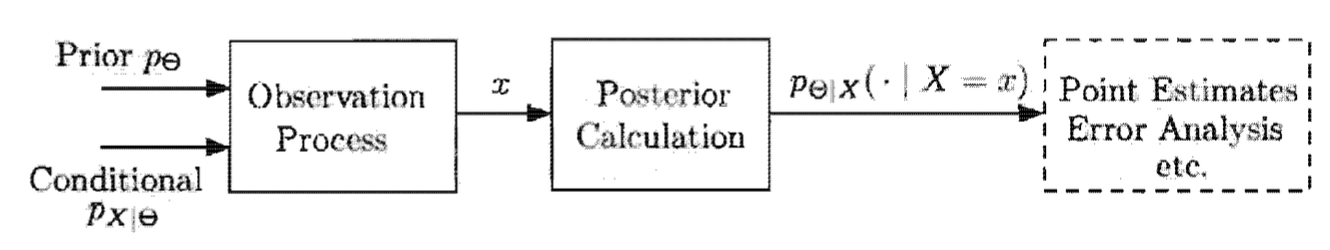
\includegraphics[width=0.8\linewidth]{figs/贝叶斯推断模型.png}
    \caption{贝叶斯推断模型}
    \label{fig:bayesian-inference}
\end{figure}

记感兴趣的未知量为 $\Theta$，并视其为一个随机变量或随机变量的有限集合。我们的目标是基于观测到的相关随机变量的值 $X=(X_1,\ldots,X_n)$ 来提取 $\Theta$ 的信息。假定已知先验分布 $p_\Theta$ 或 $f_\Theta$，以及条件分布 $p_{X\vert\Theta}$ 或 $f_{X\vert\Theta}$，则贝叶斯推断问题由 $\Theta$ 的后验分布 $p_{\Theta\vert X}$ 或 $f_{\Theta\vert X}$ 完全决定。后验分布可根据贝叶斯公式计算。
% 根据 $\Theta$ 和 $X$ 的离散性和连续性，贝叶斯公式由四种组合方式：
% \begin{gather*}
% p_{\Theta\vert X}(\theta\vert x)=\frac{p_\Theta(\theta)p_{X\vert\Theta}(x\vert\theta)}{\sum_{\theta'}p_\Theta(\theta')p_{X\vert\Theta}(x\vert\theta')},\qquad\text{$\Theta$ 离散，$X$ 离散}\\
% p_{\Theta\vert X}(\theta\vert x)=\frac{p_\Theta(\theta)f_{X\vert\Theta}(x\vert\theta)}{\sum_{\theta'}p_\Theta(\theta')f_{X\vert\Theta}(x\vert\theta')},\qquad\text{$\Theta$ 离散，$X$ 连续}\\
% f_{\Theta\vert X}(\theta\vert x)=\frac{f_\Theta(\theta)p_{X\vert\Theta}(x\vert\theta)}{\int f_\Theta(\theta')p_{X\vert\Theta}(x\vert\theta')\mathrm d\theta'},\qquad\text{$\Theta$ 连续，$X$ 离散}\\
% f_{\Theta\vert X}(\theta\vert x)=\frac{f_\Theta(\theta)f_{X\vert\Theta}(x\vert\theta)}{\int f_\Theta(\theta')f_{X\vert\Theta}(x\vert\theta')\mathrm d\theta'},\qquad\text{$\Theta$ 连续，$X$ 连续}
% \end{gather*}

\begin{example}[正态随机变量公共均值的推断]
\label{ex:normal-mean-infer}
设随机变量观测值 $X=(X_1,\ldots,X_n)$ 具有相同的未知均值。假设在给定均值的条件下，$X_i$ 是正态的，且相互独立，方差分别为 $\sigma_1^2,\ldots,\sigma_n^2$. 又设 $X_i$ 的公共均值为随机变量 $\Theta$，且先验分布为正态分布 $N(x_0,\sigma_0^2)$. 那么：
\begin{gather*}
f_\Theta(\theta)=c_1\cdot\exp\left(-\frac{(\theta-x_0)^2}{2\sigma_0^2}\right)\\
f_{X\vert\Theta}(x\vert\theta)=c_2\cdot\exp\left(-\frac{(x_1-\theta)^2}{2\sigma_1^2}\right)\cdots\exp\left(-\frac{(x_n-\theta)^2}{2\sigma_n^2}\right)
\end{gather*}
其中 $c_1,c_2$ 为常数。根据贝叶斯公式，有：
\begin{align*}
f_{\Theta\vert X}(\theta\vert x)\propto f_\Theta(\theta)f_{X\vert\Theta}(x\vert\theta)\propto\exp\left(-\sum_{i=0}^n\frac{(\theta-x_i)^2}{2\sigma_i^2}\right)\propto\exp\left(-\frac{(\theta-m)^2}{2v}\right)
\end{align*}
其中根据配方可得：
\[
m=\frac{\sum_{i=0}^nx_i/\sigma_i^2}{\sum_{i=0}^n1/\sigma_i^2},\quad v=\frac{1}{\sum_{i=0}^n1/\sigma_i^2}
\]
于是 $\Theta$ 的后验分布就是以 $m$ 为均值、$v$ 为方差的正态分布。
\end{example}

\begin{definition}[共轭分布]
在贝叶斯推断中，若先验分布与后验分布属于同一个分布族，则称先验分布与后验分布互为共轭分布。
\end{definition}
\begin{com}
例 \ref{ex:normal-mean-infer} 表明正态分布与其自身是共轭分布。这并不是一个普遍的情形，除了正态分布以外，其他常见的与自身共轭的分布有伯努利分布和二项分布。
\end{com}


\subsection{点估计，假设检验，最大后验概率准则}

\paragraph{点估计}
给定 $X$ 的观测值 $x$，贝叶斯推断给出了后验分布 $p_{\Theta\vert X}(\theta\vert x)$ 或 $f_{\Theta\vert X}(\theta\vert x)$. 后验分布包含了 $x$ 提供的所有信息，但有时我们希望得到一个数而不是一个概率分布，这就是点估计。具体而言，点估计指从 $X$ 的观测值中提取一个数 $\hat\theta=g(x)$ 作为对 $\Theta$ 的估计的方法。

\begin{definition}[估计量，估计值]
设 $g$ 是一个关于 $X$ 的函数，则称随机变量 $\hat\Theta=g(X)$ 为估计量。当观测到 $X$ 的值 $x$ 后，则称 $\hat\Theta$ 的取值 $\hat\theta=g(x)$ 为估计值。不同的函数 $g$ 引出不同的估计量。
\end{definition}

\begin{definition}[最大后验概率估计量]
给定 $X$ 的观测值 $x$，选择使得后验概率最大的 $\theta$ 作为估计值，即：
\[
\hat\theta=\max_\theta p_{\Theta\vert X}(\theta\vert x)\;\text{或}\;\max_\theta f_{\Theta\vert X}(\theta\vert x)
\]
\end{definition}

\begin{definition}[条件期望估计量]
给定 $X$ 的观测值 $x$，选择条件期望作为估计值，即：
\[
\hat\theta=\E[\Theta\vert X=x]
\]
\end{definition}
\begin{com}
在下一节中将看到，条件期望估计量其实是最小均方估计量。
\end{com}

\begin{example}[正态随机变量公共均值的估计量]
\label{ex:normal-mean-estimate}
在例 \ref{ex:normal-mean-infer} 中，我们得到了正态随机变量公共均值 $\Theta$ 的后验分布是以 $m$ 为均值、$v$ 为方差的正态分布，其中：
\[
m=\frac{\sum_{i=0}^nx_i/\sigma_i^2}{\sum_{i=0}^n1/\sigma_i^2},\quad v=\frac{1}{\sum_{i=0}^n1/\sigma_i^2}
\]
由于正态分布的概率密度函数在均值处取最大值，所以最大后验概率估计为：
\[
\hat\theta=m
\]
而正态分布的均值参数正是其期望，因此条件期望估计也为：
\[
\hat\theta=\E[\Theta\vert X=x]=m
\]
因此在该模型中，最大后验概率估计和条件期望估计恰好相同。
\end{example}

\paragraph{假设检验}
在一个假设检验问题中，$\Theta$ 取 $\theta_1,\ldots,\theta_m$ 中的一个值，其中 $m$ 是一个较小的整数（常常是 $m=2$）。称事件 $H_i=\{\Theta=\theta_i\}$ 为第 $i$ 个假设。观测到 $X$ 的取值 $x$ 后，我们希望依据某种准则选出一个最“合理”的假设。

\begin{definition}[假设检验的最大后验概率准则]
给定观测值 $x$，最大后验概率准则选择使得后验概率 $\Pb(\Theta=\theta_i\vert X=x)$ 最大的假设 $H_i$：
\[
\arg\max_i\;\Pb(\Theta=\theta_i\vert X=x)
\]
根据贝叶斯公式，这等价于：
\begin{gather*}
    \arg\max_i\;p_\Theta(\theta_i)p_{X\vert\Theta}(x\vert\theta_i),\quad\text{$X$ 离散}\\
    \arg\max_i\;p_\Theta(\theta_i)f_{X\vert\Theta}(x\vert\theta_i),\quad\text{$X$ 连续}
\end{gather*}
\end{definition}
\begin{com}
对任意观测值 $x$，最大后验概率准则是错误率最小的决策准则。
\end{com}


\subsection{贝叶斯最小均方估计}

\begin{theorem}[最小均方估计——无观测值情形]
\label{thm:lms-not-given-x}
考虑在没有观测值的情况下，用常数 $\hat\theta$ 去估计 $\Theta$，则使得均方误差 $\E[(\Theta-\hat\theta)^2]$ 最小的估计为：
\[\hat\theta=\E\Theta\]
换句话说，有：
\[
\E[(\Theta-\E\Theta)^2]\leq\E[(\Theta-\hat\theta)^2],\quad\forall\,\hat\theta
\]
\end{theorem}
\begin{proof}
对任何估计 $\hat\theta$，有均方误差：
\[
\E[(\Theta-\hat\theta)^2]=\var(\Theta-\hat\theta)+(\E[\Theta-\hat\theta])^2=\var(\Theta)+(\E\Theta-\hat\theta)^2
\]
由于 $\var(\Theta)$ 与 $\hat\theta$ 无关，故当 $(\E\Theta-\hat\theta)^2$ 最小时均方误差最小，也即 $\hat\theta=\E\Theta$.
\end{proof}

\begin{theorem}[最小均方估计——给定观测值情形]
\label{thm:lms-given-x}
设给定观测值 $x$，则使得均方误差 $\E[(\Theta-\hat\theta)^2\vert X=x]$ 最小的估计为条件期望估计：
\[\hat\theta=\E[\Theta\vert X=x]\]
换句话说，有：
\[
\E[(\Theta-\E[\Theta\vert X=x])^2\vert X=x]\leq\E[(\Theta-\hat\theta)^2\vert X=x],\quad\forall\,\hat\theta
\]
\end{theorem}
\begin{proof}
在定理 \ref{thm:lms-not-given-x} 的证明中加入 $X=x$ 的条件即可。
\end{proof}

\begin{theorem}[最小均方估计——总体情形]
\label{thm:lms-overall}
总体上，设估计量为 $\hat\Theta$，则使得均方误差 $\E[(\Theta-\hat\Theta)^2]$ 最小的估计量为：
\[
\hat\Theta=\E[\Theta\vert X]
\]
换句话说，有：
\[
\E[(\Theta-\E[\Theta\vert X])^2]\leq \E[(\Theta-\hat\Theta)^2],\quad\forall\,\hat\Theta=g(X)
\]
\end{theorem}
\begin{proof}
对于任意给定 $X$ 的取值 $x$，$\hat\theta=g(x)$ 是一个数，因此：
\[
\E[(\Theta-\E[\Theta\vert X=x])^2\vert X=x]\leq\E[(\Theta-g(x))^2\vert X=x]
\]
根据 $x$ 的任意性，有：
\[
\E[(\Theta-\E[\Theta\vert X])^2\vert X]\leq\E[(\Theta-g(X))^2\vert X]
\]
根据全期望公式，两边取期望得：
\[
\E[(\Theta-\E[\Theta\vert X])^2]\leq\E[(\Theta-g(X))^2]
\]
\end{proof}

\begin{property}
将最小均方估计和估计误差分别记为：
\[
\hat\Theta=\E[\Theta\vert X],\quad\tilde\Theta=\hat\Theta-\Theta
\]
在 \ref{sec:cond-e-cond-var} 节中已经推导了一些性质，这里列举如下：
\begin{itemize}
    \item $\hat\Theta$ 是无偏的，即 $\E[\tilde\Theta]=0$，并且 $\E[\tilde\Theta\vert X=x]=0,\,\forall\,x$
    \item 估计误差 $\tilde\Theta$ 与估计量 $\hat\Theta$ 不相关：
    $\cov(\hat\Theta,\tilde\Theta)=0$
    \item $\Theta$ 的方差可以分解为：
    $\var(\Theta)=\var(\hat\Theta)+\var(\tilde\Theta)$
\end{itemize}
\end{property}

\begin{theorem}[推广到多观测情形]
设有多个观测量 $X_1,\ldots,X_n$，则最小均方估计为：
\[
\hat\Theta=\E[\Theta\vert X_1,\ldots,X_n]
\]
换句话说，有：
\[
\E[(\Theta-\E[\Theta\vert X_1,\ldots,X_n])^2]\leq\E[(\Theta-\hat\Theta)^2],\quad\forall\,\hat\Theta=g(X_1,\ldots,X_n)
\]
\end{theorem}

\subsection{贝叶斯线性最小均方估计}
\label{sec:bayesian-lms}

\begin{definition}[线性估计量]
限定 $g$ 是关于 $X$ 的线性函数 $g(X)=aX+b$，称随机变量：
\[\hat\Theta=g(X)=aX+b\]
为线性估计量。进一步地，若有多个观测量 $X_1,\ldots,X_n$，则线性估计量的形式为：
\[\hat\Theta=a_1X_1+\cdots+a_nX_n+b\]
\end{definition}

\begin{theorem}[线性最小均方估计]
\label{thm:linear-lms-estimate}
基于 $X$ 的 $\Theta$ 的线性最小均方估计是：
\[
\hat\Theta=\E\Theta+\frac{\cov(\Theta,X)}{\var(X)}(X-\E X)=\E\Theta+\rho\frac{\sigma_\Theta}{\sigma_X}(X-\E X)
\]
其中 $\rho=\dfrac{\cov(\Theta,X)}{\sigma_\Theta\sigma_X}$ 是相关系数，此时所得均方误差为：
\[
\E[(\Theta-aX-b)^2]=(1-\rho^2)\sigma_\Theta^2
\]
\end{theorem}
\begin{proof}
假设固定 $a$，则问题等价于选择常数 $b$ 来估计随机变量 $\Theta-aX$. 根据之前的讨论，最优解为：
\[
b=\E[\Theta-aX]=\E\Theta-a\E X
\]
因此问题转化为：
\[
\min_a\;\E[(\Theta-aX-\E[\Theta-aX])^2]=\var(\Theta-aX)
\]
打开方差：
\[
\var(\Theta-aX)=\var(\Theta)+\var(aX)-2\cov(\Theta,aX)=\sigma_\Theta^2+a^2\sigma_X^2-2a\rho\sigma_\Theta\sigma_X
\]
这是关于 $a$ 的二次函数，最小值在顶点处取得：
\[
a=\frac{\rho\sigma_\Theta\sigma_X}{\sigma_X^2}=\rho\frac{\sigma_\Theta}{\sigma_X}
\]
因此线性最小均方估计为：
\[
\hat\Theta=aX+b=aX+\E\Theta-a\E X=\E\Theta+\rho\frac{\sigma_\Theta}{\sigma_X}(X-\E X)
\]
且估计误差为：
\[
\var(\Theta-aX)=\sigma_\Theta^2+a^2\sigma_X^2-2a\rho\sigma_\Theta\sigma_X=\sigma_\Theta^2+\rho^2\sigma_\Theta^2-2\rho^2\sigma_\Theta^2=(1-\rho^2)\sigma_\Theta^2
\]
\end{proof}
\begin{remark}
直观上，估计量以 $\E\Theta$ 为基础，通过 $X-\E X$ 的取值来调整。例如，不妨假设 $\rho>0$，则当观测到比 $\E X$ 更大的 $X$ 取值后，我们对 $\Theta$ 的估计也就相应地提高。另外，当 $|\rho|$ 接近 1 时，$X$ 和 $\Theta$ 高度相关，了解 $X$ 将帮助我们准确地估计 $\Theta$，因此均方误差较小。
\end{remark}

\begin{example}[正态随机变量公共均值的估计量-续]
在例 \ref{ex:normal-mean-estimate} 中，我们得到正态随机变量公共均值的最小均方估计（条件期望估计）为：
\[
\hat\theta=\E[\Theta\vert X=x]=m=\frac{\sum_{i=0}^nx_i/\sigma_i^2}{\sum_{i=0}^n1/\sigma_i^2}
\]
注意到上式是观测值 $x_1,\ldots,x_n$ 的线性组合，因此它其实也是线性最小均方估计。也即，在该模型中，最大后验概率估计、最小均方估计和线性最小均方估计恰好都是相同的。
\end{example}
 \newpage
\section{经典统计推断}

经典统计推断认为未知参数 $\theta$ 是确定的，观测 $X$ 是随机的，根据 $\theta$ 取值的不同服从 $p_X(x;\theta)$ 或 $f_X(x;\theta)$. 因此，我们将同时处理多个候选模型，每个模型对应 $\theta$ 的一个可能的取值。

\begin{figure}[H]
    \centering
    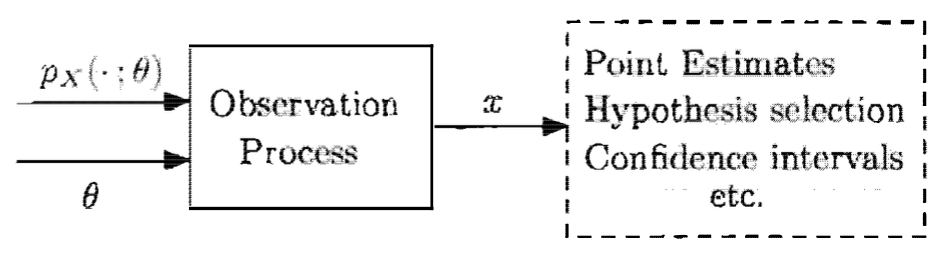
\includegraphics[width=0.5\linewidth]{figs/经典推断模型.png}
    \caption{经典推断模型}
    \label{fig:classical-inference}
\end{figure}


\subsection{经典参数估计}

\begin{definition}[估计量，估计值]
给定观测 $X=(X_1,\ldots,X_n)$，估计量指形如 $\hat\Theta_n=g(X)$ 的随机变量，估计量的取值称为估计值。注意，由于 $X$ 的分布依赖于参数 $\theta$，因而 $\hat\Theta_n$ 的分布也依赖于 $\theta$. 记 $\hat\Theta_n$ 的期望为 $\E_\theta[\hat\Theta_n]$，方差为 $\var_\theta(\hat\Theta_n)$.
\end{definition}

\begin{definition}[估计误差，偏差]
设 $\hat\Theta_n$ 是未知参数 $\theta$ 的一个估计量，定义估计误差为 $\tilde\Theta_n=\hat\Theta_n-\theta$，并定义偏差为估计误差的期望 $b_\theta(\tilde\Theta_n)=\E_\theta[\hat\Theta_n]-\theta$.
\end{definition}

\begin{definition}[无偏，渐近无偏]
若 $\E_\theta[\hat\Theta_n]=\theta$ 对 $\theta$ 所有可能的取值都成立，则称 $\hat\Theta_n$ 是无偏的；若 $\lim_{n\to\infty}\E_\theta[\hat\Theta_n]=\theta$ 对 $\theta$ 所有可能的取值都成立，则称$\hat\Theta_n$ 是渐近无偏的。
\end{definition}

\begin{definition}[相合]
若对 $\theta$ 所有可能的取值，序列 $\hat\Theta_n$ 依概率收敛到参数 $\theta$ 的真值，则称 $\hat\Theta_n$ 是 $\theta$ 的相合估计序列。
\end{definition}

\begin{property}
均方误差、偏差和 $\hat\Theta_n$ 的方差有关系：
\[
\E_\theta[\tilde\Theta_n^2]=b_\theta^2(\hat\Theta_n)+\var_\theta(\hat\Theta_n)
\]
\end{property}
\begin{remark}
这个公式很重要，等式右侧的两项体现了偏差与方差之间的权衡。
\end{remark}

\begin{definition}[极大似然估计，似然函数]
设观测向量 $X=(X_1,\ldots,X_n)$ 的联合 PMF/PDF 为 $p_X(x;\theta)$ 或 $f_X(x;\theta)$，其中 $x=(x_1,\ldots,x_n)$ 为 $X$ 的观测值。极大似然估计是使得 $p_X(x;\theta)$ 或 $f_X(x;\theta)$ 达到最大的参数值，即：
\[
\hat\theta_n=\arg\max_\theta\;p_X(x;\theta)\;\text{或}\;\arg\max_\theta\;f_X(x;\theta)
\]
称 $p_X(x;\theta)$ 或 $f_X(x;\theta)$ 为似然函数，称 $\ln p_X(x;\theta)$ 或 $\ln f_X(x;\theta)$ 为对数似然函数。
\end{definition}

\begin{remark}[极大似然估计与最大后验概率估计]
在贝叶斯最大后验概率估计中，估计的选择是使得 $p_\Theta(\theta)p_{X\vert\Theta}(x\vert\theta)$ 达到最大的 $\theta$，其中 $p_\Theta(\theta)$ 是未知参数 $\theta$ 的先验分布。因此，最大似然估计可以解释为具有均匀先验分布的最大后验概率估计。
\end{remark}

\begin{theorem}[极大似然估计的不变原理]
设 $\hat\Theta_n$ 是 $\theta$ 的极大似然估计，那么对于任意关于 $\theta$ 的一一映射函数 $h$，$h(\hat\Theta)$ 是 $\zeta=h(\theta)$ 的极大似然估计。
\end{theorem}

\begin{example}[随机变量均值的估计]
设观测值 $X_1,\ldots,X_n$ 独立同分布，均值为未知参数 $\theta$，定义样本均值为：
\[
M_n=\frac{X_1+\cdots+X_n}{n}
\]
由于 $\E_\theta[M_n]=\E_\theta[X]=\theta$，故样本均值是 $\theta$ 的无偏估计。进一步地，根据弱大数定律，$M_n$ 依概率收敛到 $\theta$，因此具有相合性。
\end{example}

\begin{example}[随机变量方差的估计]
设观测值 $X_1,\ldots,X_n$ 独立同分布，方差为未知参数 $v$，则有两个常用估计量：
\[
\bar S_n^2=\frac{1}{n}\sum\limits_{i=1}^n (X_i-M_n)^2,\qquad\hat S_n^2=\frac{1}{n-1}\sum\limits_{i=1}^n (X_i-M_n)^2
\]
可以证明 $\bar S^2$ 是有偏但渐近无偏的，$\hat S^2$ 则是无偏的。
\end{example}
\begin{proof}
注意到 $\E_{(\theta,v)}[M_n]=\theta,\,\E_{(\theta,v)}[X_i^2]=v+\theta^2,\,\E_{(\theta,v)}[M_n^2]=\frac{v}{n}+\theta^2$，于是：
\begin{align*}
\E_{(\theta,v)}[\bar S_n^2]&=\E_{(\theta,v)}\left[\frac{1}{n}\sum_{i=1}^n(X_i-M_n)^2\right]\\
&=\E_{(\theta,v)}\left[\frac{1}{n}\sum_{i=1}^nX_i^2-\frac{2M_n}{n}\sum_{i=1}^nX_i+M_n^2\right]\\
&=\E_{(\theta,v)}\left[\frac{1}{n}\sum_{i=1}^nX_i^2-2M_n^2+M_n^2\right]\\
&=v+\theta^2-\left(\frac{v}{n}+\theta^2\right)\\
&=\frac{n-1}{n}v
\end{align*}
由于 $n\to\infty$ 时 $\E_{(\theta,v)}[\bar S_n^2]\to v$，故 $\bar S_n^2$ 是渐近无偏的。又：
\[
\E_{(\theta,v)}[\hat S_n^2]=\E_{(\theta,v)}[\frac{n}{n-1}\bar S_n^2]=v
\]
故 $\hat S_n^2$ 是无偏的。
\end{proof}

\paragraph{区间估计}
在前文中，无论是贝叶斯推断中的最大后验概率估计、最小均方估计，还是经典推断中的极大似然估计，这些方法都是点估计，即给出一个数作为估计量。但有时我们还想建立一个置信区间，这就是区间估计。具体而言，我们首先固定一个\textbf{置信度} $1-\alpha$，其中 $\alpha$ 是一个很小的数。然后用一个略小的估计量 $\hat\Theta_n^-$ 和一个略大的估计量 $\hat\Theta_n^+$ 代替点估计量 $\hat\Theta_n$，使得：
\[
\Pb_\theta(\hat\Theta_n^-\leq\theta\leq\hat\Theta_n^+)\geq1-\alpha
\]
对 $\theta$ 所有可能的取值都成立。称 $[\hat\Theta_n^-,\hat\Theta_n^+]$ 为\textbf{置信区间}。

\begin{example}[正态随机变量公共均值的区间估计]
\label{ex:normal-mean-interval}
设观测量 $X_1,\ldots,X_n$ 独立同分布于 $N(\theta,v)$，其中均值 $\theta$ 未知，方差 $v$ 已知。根据例 \ref{ex:ind-normal-sum} 的结论（独立正态随机变量之和仍是正态的），可知样本均值估计量：
\[
\hat\Theta_n=\frac{X_1+\cdots+X_n}{n}\sim N\left(\theta,\frac{v}{n}\right)
\]
取 $\alpha=0.05$，即置信度 $0.95$，查正态分布表可得 $\Phi(1.96)=0.975=1-\alpha/2$，于是：
\[
\Pb_\theta\left(\left|\frac{\hat\Theta_n-\theta}{\sqrt{v/n}}\right|\leq1.96\right)=\Pb_\theta\left(\hat\Theta_n-1.96\sqrt{\frac{v}{n}}\leq\theta\leq \hat\Theta_n+1.96\sqrt{\frac{v}{n}}\right)=0.95
\]
这说明：
\[
\left[\hat\Theta_n-1.96\sqrt{\frac{v}{n}},\;\hat\Theta_n+1.96\sqrt{\frac{v}{n}}\right]
\]
是 $95\%$ 置信区间。
\end{example}

\begin{example}[基于方差近似估计量的区间估计]
设观测量 $X_1,\ldots,X_n$ 独立同分布于 $N(\theta,v)$，其中均值 $\theta$ 和方差 $v$ 都是未知的。考虑用方差的无偏估计量：
\[
\hat S_n^2=\frac{1}{n-1}\sum_{i=1}^n(X_i-\hat\Theta_n)^2
\]
代替方差，则根据例 \ref{ex:normal-mean-interval} 和中心极限定理，可构造一个近似的 $1-\alpha$ 置信区间：
\[
\left[\hat\Theta_n-z\frac{\hat S_n}{\sqrt{n}},\;\hat\Theta_n+z\frac{\hat S_n}{\sqrt{n}}\right]
\]
其中 $z$ 满足 $\Phi(z)=1-\alpha/2$. 例如，近似 $95\%$ 置信区间为：
\[
\left[\hat\Theta_n-1.96\frac{\hat S_n}{\sqrt{n}},\;\hat\Theta_n+1.96\frac{\hat S_n}{\sqrt{n}}\right]
\]
事实上，当用 $\hat S_n^2$ 代替方差后，随机变量：
\[
T_n=\frac{\sqrt{n}(\hat\Theta_n-\theta)}{\hat S_n}
\]
服从自由度为 $n-1$ 的 $t$ 分布（详见附录 \ref{sec:normal-derive}）。因此，设 $t$ 分布的分布函数为 $\Psi_{n-1}(z)$，则更精确的置信区间中，$z$ 应满足 $\Psi_{n-1}(z)=1-\alpha/2$. 
\end{example}

\begin{definition}[充分统计量]
给定观测 $X=(X_1,\ldots,X_n)$，设随机变量 $T=q(X)$ 为 关于 $X$ 的标量或向量函数，若 $X$ 在给定 $T$ 下的条件分布不依赖于 $\theta$，即：
\[
\Pb_\theta(X\in D\vert T=t),\quad\forall\,t
\]
对所有 $\theta$ 都是一样的，则称 $T$ 为 $\theta$ 的充分统计量。
\end{definition}

\begin{theorem}[因子分解定理]
\label{thm:factorization}
$T=q(X)$ 是 $\theta$ 的充分统计量当且仅当似然函数 $p_X(x;\theta)$ 或 $f_X(x;\theta)$ 可以写成 $r(q(x),\theta)s(x)$ 的形式，其中 $r,s$ 是两个函数。
\end{theorem}
\begin{proof}
假设 $X$ 是离散随机变量，连续情形类似。首先证明充分性。假设 $p_X(x;\theta)=r(q(x),\theta)s(x)$，取定 $T=t$，则对所有 $q(x)\neq t$ 的 $x$，容易知道：
\[
\Pb_\theta(X=x\vert T=t)=\frac{\Pb_\Theta(X=x)\Pb_\theta(T=t\vert X=x)}{\Pb_\theta(T=t)}=0
\]
而对于满足 $q(x)=t$ 的 $x$，有：
\begin{align*}
\Pb_\theta(X=x\vert T=t)&=\frac{\Pb_\theta(X=x,T=t)}{\Pb_\theta(T=t)}=\frac{\Pb_\theta(X=x)}{\Pb_\theta(T=t)}=\frac{\Pb_\theta(X=x)}{\sum_z\Pb_\theta(X=z,T=t)}\\
&=\frac{\Pb_\theta(X=x)}{\sum_{\{z\mid q(z)=t\}}\Pb_\theta(X=z)}=\frac{r(q(x),\theta)s(x)}{\sum_{\{z\mid q(z)=t\}}r(q(z),\theta)s(z)}\\
&=\frac{r(t,\theta)s(x)}{r(t,\theta)\sum_{\{z\mid q(z)=t\}}s(z)}=\frac{s(x)}{\sum_{\{z\mid q(z)=t\}}s(z)}
\end{align*}
可见对所有 $x$，$\Pb_\theta(X=x\vert T=t)$ 都不依赖于 $\theta$，故 $T$ 是充分统计量。

然后证明必要性。设 $T=q(X)$ 是 $\theta$ 的充分统计量，则对任意 $x$，有：
\[
p_X(x;\theta)=\sum_t\Pb_\theta(X=x\vert T=t)\Pb_\theta(T=t)=\Pb_\theta(X=x\vert T=q(x))\Pb_\theta(T=q(x))
\]
右式两部分中，前者与 $\theta$ 无关，故可写作 $s(x)$ 的形式，而后者为 $r(q(x),\theta)$ 的形式。
\end{proof}

\begin{theorem}
若 $q(X)$ 是 $\theta$ 的充分统计量，则对 $\theta$ 的任何函数 $h$，$q(X)$ 都是 $\zeta=h(\theta)$ 的充分统计量。
\end{theorem}
\begin{proof}
对 $\zeta=h(\theta)$ 有：
\[
\Pb_{\zeta}(X\in D\vert T=t)=\Pb_{\theta}(X\in D\vert T=t)
\]
所以 $\Pb_{\zeta}(X\in D\vert T=t)$ 对所有 $\zeta$ 都是一样的。
\end{proof}

\begin{theorem}
若 $q(X)$ 是 $\theta$ 的充分统计量，则 $\theta$ 的极大似然估计可以写作 $\hat\Theta_n=\phi(q(X))$.
\end{theorem}
\begin{proof}
根据因子分解定理 \ref{thm:factorization}，$p_X(x;\theta)=r(q(x),\theta)s(x)$，故极大似然估计为：
\[
\hat\theta_n=\arg\max_\theta\;p_X(x;\theta)=\begin{dcases}
    \arg\max_\theta\;r(q(x),\theta),&\text{$s(x)>0$}\\
    \arg\min_\theta\;r(q(x),\theta),&\text{$s(x)<0$}
\end{dcases}
\]
即 $\hat\theta_n$ 只通过 $\phi(q(x))$ 依赖于 $x$，故 $\hat\Theta_n=\phi(q(X))$.
\end{proof}
\begin{remark}
该定理说明充分统计量抓住了由 $X$ 提供的关于 $\theta$ 的所有核心信息。
\end{remark}

\begin{example}[伯努利分布]
设 $X_1,\ldots,X_n$ 独立同分布于参数为 $\theta$ 的伯努利分布，则：
\[
q(X)=\sum_{i=1}^nX_i
\]
是 $\theta$ 的充分统计量。这是因为似然函数为：
\[
p_X(x;\theta)=\theta^{\sum_{i=1}^n x_i}(1-\theta)^{n-\sum_{i=1}^nx_i}=\theta^{q(x)}(1-\theta)^{n-q(x)}
\]
可以分解为 $r(q(x),\theta)=\theta^{q(x)}(1-\theta)^{n-q(x)}$ 与常函数 $s(x)=1$ 的乘积。
\end{example}

\begin{example}[泊松分布]
设 $X_1,\ldots,X_n$ 独立同分布于参数为 $\theta$ 的泊松分布，则：
\[
q(X)=\sum_{i=1}^nX_i
\]
是 $\theta$ 的充分统计量。这是因为似然函数为：
\[
p_X(x;\theta)=\prod_{i=1}^np_{X_i}(x_i;\theta)=e^{-\theta}\prod_{i=1}^n\frac{\theta^{x_i}}{x_i!}=e^{-\theta}\frac{\theta^{q(x)}}{\prod_{i=1}^nx_i!}
\]
可以分解为 $r(q(x),\theta)=e^{-\theta}\theta^{q(x)}$ 与 $s(x)=1/\prod_{i=1}^nx_i!$ 的乘积。
\end{example}

\begin{example}[正态分布]
设 $X_1,\ldots,X_n$ 独立同分布于 $N(\mu,\sigma^2)$，则：
\begin{itemize}
    \item 若 $\sigma^2$ 已知，则 $q(X)=\sum_{i=1}^nX_i$ 是 $\mu$ 的充分统计量。
    \item 若 $\mu$ 已知，则 $q(X)=\sum_{i=1}^n(X_i-\mu)^2$ 是 $\sigma^2$ 的充分统计量。
    \item 若 $\mu,\sigma^2$ 都未知，则 $q(X)=(\sum_{i=1}^nX_i,\sum_{i=1}^nX_i^2)$ 是 $(\mu,\sigma^2)$ 的充分统计量。
\end{itemize}
\end{example}

\begin{theorem}[Rao-Blackwell]
给定观测 $X=(X_1,\ldots,X_n)$，设 $T=q(X)$ 是参数 $\theta$ 的充分统计量，$g(X)$ 是 $\theta$ 的一个估计量。则：
\begin{enumerate}
    \item $\E_\theta[g(X)\vert T]$ 对所有 $\theta$ 都一样，因而可以去掉下标 $\theta$，将：
    \[
    \hat g(X)=\E[g(X)\vert T]
    \]
    视作 $\theta$ 的一个新估计量，它只通过 $T$ 依赖于 $X$.
    \item 新估计量 $\hat g(X)$ 与原估计量 $g(X)$ 偏差相等。
    \item 对满足 $\var_\theta(g(X))<\infty$ 的 $\theta$，有均方误差：
    \[
    \E_\theta[(\hat g(X)-\theta)^2]\leq\E_\theta[(g(X)-\theta)^2]
    \]
    进一步地，给定 $\theta$，此不等式是严格的当且仅当：
    \[
    \E_\theta[\var(g(X)\vert T)]>0
    \]
\end{enumerate}
\end{theorem}
\begin{proof}
我们逐条证明：
\begin{enumerate}
    \item 由于 $T$ 是充分估计量，所以条件分布 $\Pb_\theta(X=x\vert T=t)$ 不依赖于 $\theta$，自然 $\E_\theta[g(X)\vert T]$ 不依赖于 $\theta$.
    \item 根据全期望公式，有：
    \[
    \E_\theta[\hat g(X)]=\E[\E[g(X)\vert T]]=\E_\theta[g(X)]
    \]
    因而偏差相等：
    \[
    \E_\theta[\hat g(x)]-\theta=\E_\theta[g(x)]-\theta
    \]
    \item 对于固定的 $\theta$，记 $\hat g(X)$ 和 $g(X)$ 的偏差为 $b_\theta$. 根据全方差公式，有：
    \begin{align*}
    \E_\theta[(g(X)-\theta)^2]&=\var_\theta(g(X))+b_\theta^2\\
    &=\E_\theta[\var(g(X)\vert T)]+\var_\theta(\E[g(X)\vert T])+b_\theta^2\\
    &=\E_\theta[\var(g(X)\vert T)]+\var_\theta(\hat g(X))+b_\theta^2\\
    &=\E_\theta[\var(g(X)\vert T)]+\E_\theta[(\hat g(X)-\theta)^2]\\
    &\geq\E_\theta[(\hat g(X)-\theta)^2]
    \end{align*}
    且不等式是严格的当且仅当 $\E_\theta[\var(g(X)\vert T)]>0$.
\end{enumerate}
\end{proof}
\begin{remark}
Rao-Blackwell 定理说明，一个一般的估计量可以改进为一个只依赖于充分统计量的估计量，新估计量与原估计量的偏差相同，但均方误差更小。
\end{remark}

\begin{example}
设 $X_1,\ldots,X_n$ 是 $[0,\theta]$ 上独立同分布的均匀随机变量。
\begin{enumerate}[label=(\alph*)]
    \item 证明 $T=\max_{i=1,\ldots,n}X_i$ 是充分统计量。
    \item 证明 $g(X)=(2/n)\sum_{i=1}^nX_i$ 是无偏估计。
    \item 找出估计量 $\hat g(X)=\E[g(X)\vert T]$ 的形式，计算并比较 $\E_\theta[(\hat g(X)-\theta)^2]$ 和 $\E_\theta[(g(X)-\theta)^2]$.
\end{enumerate}
\end{example}
\begin{proof}
\,
\begin{enumerate}[label=(\alph*)]
    \item 由于似然函数为：
    \[
    f_X(x_1,\ldots,x_n;\theta)=\begin{cases}
    1/\theta^n,&0\leq \max_{i=1,\ldots,n}x_i\leq\theta\\
    0,&\text{otherwise}
    \end{cases}
    \]
    只通过 $\max_{i=1,\ldots,n}x_i$ 依赖于 $x$，根据因子分解定理可知其为充分统计量。
    \item 由于：
    \[
    \E_\theta[g(X)]=\frac{2}{n}\sum_{i=1}^n\E_\theta[X_i]=\frac{2}{n}\sum_{i=1}^n\frac{\theta}{2}=\theta
    \]
    故 $g(X)$ 是无偏估计。
    \item 固定 $T=t$，则 $X_1,\ldots,X_n$ 中有一个等于 $t$，其余观测服从 $[0,t]$ 上的均匀分布，因此：
    \[
    \E[g(X)\vert T=t]=\frac{2}{n}\E_\theta\left[\sum_{i=1}^nX_i\vert T=t\right]=\frac{2}{n}\left(t+(n-1)\frac{t}{2}\right)=\frac{n+1}{n}t
    \]
    所以：
    \[
    \hat g(X)=\E[g(X)\vert T]=\frac{n+1}{n}T
    \]
    下面计算均方误差。首先计算一阶矩：
    \[
    \E_\theta[\hat g(X)]=\E_\theta[\E[g(X)\vert T]]=\E_\theta[g(X)]=\theta
    \]
    可以看出 $\hat g(X)$ 也是无偏估计，这符合 Rao-Blackwell 定理的第二点。为了计算二阶矩，需要首先确定 $T$ 的分布：
    \[
    F_T(t;\theta)=\Pb_\theta(T\leq t)=\left(\frac{t}{\theta}\right)^n\implies f_T(t;\theta)=\frac{nt^{n-1}}{\theta^n},\quad t\in[0,\theta]
    \]
    于是：
    \[
    \E_\theta[(\hat g(X))^2]=\left(\frac{n+1}{n}\right)^2\E_\theta\left[T^2\right]=\left(\frac{n+1}{n}\right)^2\int_0^\theta t^2\frac{nt^{n-1}}{\theta^n}\mathrm dt=\frac{(n+1)^2}{n(n+2)}\theta^2
    \]
    由于 $\hat g(X)$ 是无偏估计，所以均方误差就是方差：
    \[
    \E_\theta[(\hat g(X)-\theta)^2]=\E_\theta[(\hat g(X))^2]-\theta^2=\frac{(n+1)^2}{n(n+2)}\theta^2-\theta^2=\frac{\theta^2}{n(n+2)}
    \]
    同理，$g(X)$ 均方误差也是其方差，且：
    \[
    \E_\theta[(g(X)-\theta)^2]=\var_\theta(g(X))=\frac{4}{n^2}\sum_{i=1}^n\var_\theta(X_i)=\frac{4}{n^2}\sum_{i=1}^n\frac{\theta^2}{12}=\frac{\theta^2}{3n}
    \]
    由于 $n(n+2)\geq 3n,\;\forall n>0$，所以：
    \[
    \E_\theta[(\hat g(X)-\theta)^2]\leq\E_\theta[(g(X)-\theta)^2]
    \]
    即我们得到了一个方差更小的无偏估计。这符合 Rao-Blackwell 定理的第三点。
\end{enumerate}
\end{proof}


\subsection{线性回归}

线性回归为两个或多个变量建立线性模型，可以由\textbf{最小二乘法}完成而不需要任何概率上的解释，但也可以在各种概率框架下进行解释。

\paragraph{一元线性回归}
设有 $n$ 个数据对 $(x_i,y_i),\,i=1,\ldots,n$，建立线性模型：
\[
y\approx\theta_0+\theta_1 x
\]
其中 $\theta_0,\theta_1$ 是未知的待估计参数。特别地，给定参数的估计 $\hat\theta_0,\hat\theta_1$，则模型对 $x_i$ 的估计为：
\[
\hat y_i=\hat\theta_0+\hat\theta_1 x_i
\]
其与真实值 $y_i$ 之间的差异称作残差：
\[
\tilde y_i=y_i-\hat y_i
\]
线性回归的优化目标是最小化残差的平方和：；
\[
\min_{\theta_0,\theta_1}\quad \sum_{i=1}^n(y_i-\hat y_i)^2=\sum_{i=1}^n(y_i-\theta_0-\theta_1 x_i)^2
\]
这是关于 $\theta_0,\theta_1$ 的二次函数，容易求得最优估计为：
\[
\hat\theta_1=\frac{\sum\limits_{i=1}^n(x_i-\bar x)(y_i-\bar y)}{\sum\limits_{i=1}^n(x_i-\bar x)^2},\quad\hat\theta_0=\bar y-\hat\theta_1\bar x
\]
其中，
\[
\bar x=\frac{1}{n}\sum_{i=1}^n x_i,\quad \bar y=\frac{1}{n}\sum_{i=1}^ny_i
\]

\paragraph{概率框架解释·极大似然}
对于每个 $x_i$，将 $y_i$ 视作随机变量 $Y_i$ 的一个取值。设 $Y_i$ 的模型为：
\[
Y_i=\theta_0+\theta_1 x_i+W_i,\;i=1,\ldots,n
\]
其中 $W_i$ 是均值为零、方差为 $\sigma^2$ 的正态独立同分布随机变量，因而 $Y_i$ 也是独立的正态随机变量且 $Y_i\sim N(\theta_0+\theta_1 x_i,\sigma^2)$. 于是似然函数为：
\[
f_Y(y;\theta)=\prod_{i=1}^n\frac{1}{\sqrt{2\pi}\sigma}\exp\left\{-\frac{(y_i-\theta_0-\theta_1 x_i)^2}{2\sigma^2}\right\}
\]
当似然函数最大时，指数部分达到最大，即残差平方和最小。因此最小二乘法可以视为 $Y$ 的期望具有线性结构的正态模型中参数 $\theta_0,\theta_1$ 的极大似然估计。

\paragraph{概率框架解释·近似贝叶斯线性最小均方估计}
将 $x_i,y_i$ 都视作随机变量 $X_i,Y_i$ 的取值，设不同 $(X_i,Y_i)$ 之间是独立同分布的，但是它们的二维联合分布未知。考虑服从同一分布的另一随机变量对 $(X_0,Y_0)$，假设观测到 $X_0$ 并希望用线性估计量 $\hat Y_0=\theta_0+\theta_1 X_0$ 来估计 $Y_0$. 根据定理 \ref{thm:linear-lms-estimate}，$Y_0$ 的线性最小均方估计量为：
\[
\hat Y_0=\E Y_0+\frac{\cov(Y_0,X_0)}{\var(X_0)}(X_0-\E X_0)
\]
也即：
\[
\theta_1=\frac{\cov(Y_0,X_0)}{\var(X_0)},\quad\theta_0=\E Y_0-\theta_1\E X_0
\]
由于我们不知道 $(X_0,Y_0)$ 的分布，因此作估计：
\[
    \E X_0\approx\bar x,\quad
    \E Y_0\approx\bar y,\quad
    \cov(Y_0,X_0)\approx\frac{1}{n}\sum_{i=1}^n(x_i-\bar x)(y_i-\bar y),\quad
    \var(X_0)\approx\frac{1}{n}\sum_{i=1}^n(x_i-\bar x)^2
\]
代入即可得到最小二乘公式。

\paragraph{概率框架解释·近似贝叶斯最小均方估计}

仍然假设 $(X_i,Y_i)$ 独立同分布，并附加新的假设——数据满足模型：
\[
Y_i=\theta_0+\theta_1X_i+W_i
\]
其中 $W_i$ 是独立同分布的零均值噪声项且与 $X_i$ 独立。根据定理 \ref{thm:lms-overall} 可知，$Y_0$ 的最小均方估计量为：
\[
\E[Y_0\vert X_0]=\E[\theta_0+\theta_1X_0+W_0\vert X_0]=\theta_0+\theta_1X_0
\]
换句话说，$\theta_0+\theta_1X_0$ 是所有关于 $X_0$ 的函数 $g(X_0)$ 中使得均方误差最小的，于是：
\[
\theta_0,\theta_1=\argmin_{\theta_0',\theta_1'}\;\E[(Y_0-\theta_0'-\theta_1'X_0)^2]
\]
注意到，根据弱大数定律，当 $n\to\infty$ 时，上式是：
\[
\frac{1}{n}\sum_{i=1}^n(Y_i-\theta_0'-\theta_1'X_i)^2
\]
的极限，而该式正是最小二乘法的优化目标。

\paragraph{贝叶斯线性回归}
将 $x_1,\ldots,x_n$ 视为给定的数，将 $(y_1,\ldots,y_n)$ 视为随机向量 $Y=(Y_1,\ldots,Y_n)$ 的观测值，且假设有线性关系：
\[
Y_i=\Theta_0+\Theta_1x_i+W_i
\]
其中 $\Theta=(\Theta_0,\Theta_1)$ 是待估计的参数（视为随机变量）。假设 $\Theta_0,\Theta_1,W_1,\ldots,W_n$ 是相互独立的正态随机变量。$W_1,\ldots,W_n$ 均值为零，方差已知为 $\sigma^2$. $\Theta_0,\Theta_1$ 的均值为零，方差分别为 $\sigma_0^2,\sigma_1^2$. 则根据贝叶斯公式，后验概率密度函数为：
\begin{align*}
f_{\Theta\vert Y}(\theta_0,\theta_1\vert y_1,\ldots,y_n)&\propto f_\Theta(\theta_0,\theta_1)f_{Y\vert\Theta}(y_1,\ldots,y_n\vert \theta_0,\theta_1)\\
&\propto\exp\left(-\frac{\theta_0^2}{2\sigma_0^2}\right)\cdot\exp\left(-\frac{\theta_1^2}{2\sigma_1^2}\right)\prod_{i=1}^n\cdot\exp\left(-\frac{y_i^2}{2\sigma^2}\right)\\
&\propto\exp\left(-\left(\frac{\theta_0^2}{2\sigma_0^2}+\frac{\theta_1^2}{2\sigma_1^2}+\sum_{i=1}^n\frac{y_i^2}{2\sigma^2}\right)\right)
\end{align*}
因此，最大后验概率估计就是：
\[
\hat\theta_0,\hat\theta_1=\argmin_{\theta_0,\theta_1}\;\left(\frac{\theta_0^2}{2\sigma_0^2}+\frac{\theta_1^2}{2\sigma_1^2}+\sum_{i=1}^n\frac{y_i^2}{2\sigma^2}\right)
\]
求导并令导数为零，可解得：
\[
    \hat\theta_1=\frac{\sigma_1^2}{\sigma^2+\sigma_1^2\sum_{i=1}^n(x_i-\bar x)^2}\cdot\sum_{i=1}^n(x_i-\bar x)(y_i-\bar y),\quad\hat\theta_0=\frac{n\sigma_0^2}{\sigma^2+n\sigma_0^2}(\bar y-\hat\theta_1\bar x)
\]

\paragraph{多元线性回归}
一元线性回归可以直接扩展到多元情形。例如，设数据由三元组 $(x_i,y_i,z_i)$ 组成，建立线性模型：
\[
y\approx\theta_0+\theta_1x+\theta_2z
\]
则多元线性回归最小化残差的平方和：
\[
\min_{\theta_0,\theta_1,\theta_2}\quad\sum_{i=1}^n(y_i-\theta_0-\theta_1x_i-\theta_2z_i)^2
\]

特别地，$z$ 可以是 $x$ 的函数，例如 $z=x^2$. 尽管二次函数不是线性的，但是未知参数 $\theta_j$ 与随机变量 $Y_i$ 是线性关系，所以这仍然属于线性回归的范畴。一般地，考虑如下形式的模型：
\[
y\approx\theta_0+\sum_{j=1}^m\theta_jh_j(x)
\]
则回归问题的优化目标为：
\[
\min_{\theta_0,\ldots,\theta_m}\quad\sum_{i=1}^n\left(y_i-\theta_0-\sum_{j=1}^m\theta_jh_j(x_i)\right)^2
\]
这样的最小化问题都有现存的公式。


\subsection{简单假设检验}

在经典统计推断中，我们不再有先验概率的假设，因此假设检验问题可以看作是 $\theta$ 只有两个取值的推断问题。我们一般用 $H_0$ 表示\textbf{原假设}，$H_1$ 表示\textbf{备择假设}。

设观测随机变量 $X=(X_1,\ldots,X_n)$，记 $\Pb(X\in A;H_j)$ 表示假设 $H_j$ 成立时 $X$ 属于 $A$ 的概率。类似地，记 $p_X(x;H_j)$ 或 $f_X(x;H_j)$ 表示假设 $H_j$ 成立时的 PMF 或 PDF. 我们希望找到一个决策准则将观测值 $x$ 映射到其中一个假设上去。任何一个决策准则都将样本空间划分为了两个区域——拒绝域与接受域。当观测数据落入拒绝域时，称假设 $H_0$ 被拒绝，反之则被接受。

一个决策准则有两种错误。设该决策准则决定的拒绝域为 $R$，第一类错误指拒绝了 $H_0$ 但它实际上是正确的，此类错误发生概率为 $\alpha(R)=\Pb(x\in R;H_0)$；第二类错误指接受了 $H_0$ 但它实际上是错误的，此类错误发生概率为 $\beta(R)=\Pb(x\not\in R;H_1)$.

\begin{definition}[似然比]
定义似然比为：
\[
L(x)=\frac{p_X(x;H_1)}{p_X(x;H_0)}\quad\text{或}\quad L(x)=\frac{f_X(x;H_1)}{f_X(x;H_0)}
\]
\end{definition}

基于似然比的概念，我们可以得到这样的决策准则：选择一个临界值 $\xi\in(0,\infty)$，当观测值 $x$ 满足 $L(x)>\xi$ 时，拒绝原假设 $H_0$. 特别地，当 $\xi=1$ 时，我们总是选择似然最大的假设，此时正好对应极大似然准则。

\paragraph{似然比检验}
首先确定错误拒绝的概率 $\alpha$，然后选择一个常数 $\xi$，使得错误拒绝的概率为 $\alpha$：
\[
\Pb(L(x)>\xi;H_0)=\alpha
\]
那么拒绝域就是 $R=\{x\mid L(x)>\xi\}$. 当观测值落入拒绝域中时，即 $L(x)>\xi$ 时，我们拒绝 $H_0$.

\begin{lemma}[Neyman-Pearson 引理]
考虑似然比检验中一个确定的 $\xi$，从而有犯错概率：
\[
\Pb(L(X)>\xi;H_0)=\alpha,\quad\Pb(L(X)\leq\xi;H_1)=\beta
\]
假设还有其他检验，拒绝域为 $R$，使得错误拒绝的概率一样或更小：
\[
\Pb(X\in R;H_0)\leq\alpha
\]
那么这个检验错误接受的概率一样或更大：
\[
\Pb(X\not\in R;H_1)\geq\beta
\]
当 $\Pb(X\in R;H_0)<\alpha$ 严格成立时，$\Pb(X\not\in R;H_1)>\beta$ 严格成立。
\end{lemma}


\subsection{显著性检验}

在实际情况中，假设检验问题并不总是只有两个特定的选择，因而简单假设检验的方法可能不再适用。本节介绍更一般的问题和解决方法。

假设观测 $X=(X_1,\ldots,X_n)$ 服从由参数 $\theta$ 决定的 PMF/PDF，其中 $\theta$ 在给定集合 $\mathcal M$ 中取值。我们称“断言 $\theta$ 的真值为 $\theta_0\in\mathcal M$” 为原假设，记作 $H_0$，而相应的 $\theta\neq\theta_0$ 为备择假设，记作 $H_1$.

\paragraph{显著性检验}
基于观测 $X_1,\ldots,X_n$，对假设 $H_0:\theta=\theta_0$ 做统计检验：
\begin{enumerate}
    \item 选择统计量 $S=h(X_1,\ldots,X_n)$，其中 $h:\mathbb R^n\to\mathbb R$.
    \item 确定拒绝域形状：拒绝域 $R$ 为 $S$ 的取值的子集，当 $S$ 落入 $R$ 时就拒绝 $H_0$；这个过程通常涉及一个常数 $\xi$，称作临界值；
    \item 选择显著水平 $\alpha$；
    \item 选择临界值 $\xi$ 使得错误拒绝的概率等于或约等于 $\alpha$；此时拒绝域 $R$ 就完全确定了；
    \item 得到 $X_1,\ldots,X_n$ 的观测值 $x_1,\ldots,x_n$，计算统计值 $s=h(x_1,\ldots,x_n)$，若 $s$ 落入 $R$ 则拒绝 $H_0$.
\end{enumerate}

\begin{com}
很多时候，统计学家并不选择显著水平 $\alpha$ 和临界值 $\xi$，而是计算统计值 $s$ 后，直接汇报 $p$-值：
\[
    p\text{-值}=\min\{\alpha\mid H_0\,\text{在显著水平 $\alpha$ 下被拒绝}\}
\]
\end{com}

 \newpage

\appendix
\section{常见随机变量}
\label{sec:random-variables}

本节总结常见的随机变量及其期望、方差、矩母函数和性质，其中离散随机变量包括伯努利、二项、泊松、几何和超几何随机变量，连续随机变量包括均匀、指数、柯西、伽马和正态随机变量。


\paragraph{伯努利随机变量}

\begin{itemize}[itemsep=1ex]
    \item 记号：$X\sim B(1,p)$
    \item 实例：抛掷一枚硬币，硬币向上概率为 $p$，$X$ 为是否向上。
    \item PMF：$p_X(k)=\begin{cases}p,&k=1\\1-p,&k=0\end{cases}$
    \item 期望：$\E X=p$
    \item 方差：$\var X=p(1-p)$
    \item 矩母函数：$M_X(s)=1-p+pe^s$
\end{itemize}

\begin{proof}[矩母函数的推导]
\[
M_X(s)=\E[e^{sX}]=(1-p)\cdot e^{0}+p\cdot e^{s}=1-p+pe^s
\]
\end{proof}

\paragraph{二项随机变量}

\begin{itemize}[itemsep=1ex]
    \item 记号：$X\sim B(n,p)$
    \item 实例：抛掷 $n$ 枚硬币，每枚硬币向上概率均为 $p$，$X$ 为向上次数。
    \item PMF：$p_X(k)=\displaystyle\binom{n}{k}p^k(1-p)^{n-k},\quad k=0,1,2,\ldots,n$
    \item 期望：$\E X=np$
    \item 方差：$\var X=np(1-p)$
    \item 矩母函数：$M_X(s)=(1-p+pe^s)^n$
\end{itemize}

\begin{proof}[期望的推导]
\begin{align*}
\E X&=\sum_{k=0}^{n}k\binom{n}{k}p^k(1-p)^{n-k}=\sum_{k=1}^nn\binom{n-1}{k-1}p^k(1-p)^{n-k}\\
&=np\sum_{k=0}^{n-1}\binom{n-1}{k}p^k(1-p)^{n-1-k}=np(p+1-p)^{n-1}=np
\end{align*}
其中用到了恒等式 $\displaystyle\binom{n}{k}=\binom{n-1}{k-1}\frac{n}{k}$ 和二项式定理。
\end{proof}
\begin{proof}[二阶矩的推导]
\begin{align*}
\E X^2&=\sum_{k=0}^{n}k^2\binom{n}{k}p^k(1-p)^{n-k}=\sum_{k=1}^nnk\binom{n-1}{k-1}p^k(1-p)^{n-k}\\
&=\sum_{k=1}^nn\binom{n-1}{k-1}p^k(1-p)^{n-k}+\sum_{k=1}^nn(k-1)\binom{n-1}{k-1}p^k(1-p)^{n-k}\\
&=np+np\sum_{k=0}^{n-1}k\binom{n-1}{k}p^{k}(1-p)^{n-1-k}=np+np(n-1)p
\end{align*}
\end{proof}
\begin{proof}[方差的推导]
\[
\var X=\E X^2-(\E X)^2=np+n(n-1)p^2-n^2p^2=np-np^2=np(1-p)
\]
\end{proof}
\begin{proof}[矩母函数的推导]
\[
M_X(s)=\E[e^{sX}]=\sum_{k=0}^n\binom{n}{k}p^k(1-p)^{n-k}e^{sk}=(1-p+pe^s)^n
\]
\end{proof}

\paragraph{泊松随机变量}

\begin{itemize}[itemsep=1ex]
    \item 记号：$X\sim P(\lambda)$
    \item 实例：一个城市一天中发生车祸次数。
    \item PMF：$p_X(k)=e^{-\lambda}\dfrac{\lambda^k}{k!},\quad k=0,1,\ldots$
    \item 期望：$\E X=\lambda$
    \item 方差：$\var X=\lambda$
    \item 矩母函数：$M_X(s)=e^{\lambda(e^s-1)}$
    \item 性质：取 $\lambda=np$，则当 $n\to\infty$ 时，泊松分布近似二项分布。
\end{itemize}

\begin{proof}[期望的推导]
\[
\E X=\sum_{k=0}^\infty ke^{-\lambda}\frac{\lambda^k}{k!}=e^{-\lambda}\sum_{k=1}^{\infty}\frac{\lambda^k}{(k-1)!}=\lambda e^{-\lambda}\sum_{k=0}^{\infty}\frac{\lambda^k}{k!}=\lambda
\]
其中用到了 $e^x$ 的泰勒展开。
\end{proof}
\begin{proof}[二阶矩的推导]
\begin{align*}
\E X^2&=\sum_{k=0}^\infty k^2e^{-\lambda}\frac{\lambda^k}{k!}=e^{-\lambda}\sum_{k=1}^{\infty}k\frac{\lambda^k}{(k-1)!}\\
&=e^{-\lambda}\sum_{k=1}^{\infty}\frac{\lambda^k}{(k-1)!}+e^{-\lambda}\sum_{k=2}^{\infty}\frac{\lambda^k}{(k-2)!}\\
&=e^{-\lambda}\lambda e^\lambda+e^{-\lambda}\lambda^2 e^\lambda=\lambda+\lambda^2
\end{align*}
\end{proof}
\begin{proof}[方差的推导]
\[
\var X=\E X^2-(\E X)^2=\lambda+\lambda^2-\lambda^2=\lambda
\]
\end{proof}
\begin{proof}[矩母函数的推导]
\[
M_X(s)=\E[e^{sX}]=\sum_{k=0}^\infty e^{-\lambda}\frac{\lambda^k}{k!}e^{sk}=e^{-\lambda}\sum_{k=0}^\infty \frac{(\lambda e^s)^k}{k!}=e^{\lambda(e^s-1)}
\]
\end{proof}
\begin{proof}[证明泊松分布近似二项分布]
取 $\lambda=np$，则：
\begin{align*}
\lim_{n\to\infty}\binom{n}{k}p^k(1-p)^{nk}&=\lim_{n\to\infty}\frac{n^{\underline{k}}}{k!}\cdot\frac{\lambda^k}{n^k}\left(1-\frac{\lambda}{n}\right)^{n-k}\\
&=\frac{\lambda^k}{k!}\lim_{n\to\infty}\frac{n^{\underline{k}}}{n^k}\cdot\left(1-\frac{\lambda}{n}\right)^{n-k}\\
&=\frac{\lambda^k}{k!}\cdot 1\cdot\lim_{n\to\infty}\left[\left(1-\frac{\lambda}{n}\right)^{-\frac{n}{\lambda}}\right]^{-\frac{\lambda(n-k)}{n}}\\
&=\frac{\lambda^k}{k!}e^{-\lambda}
\end{align*}
\end{proof}

\paragraph{几何随机变量}

\begin{itemize}[itemsep=1ex]
    \item 记号：$X\sim G(p)$
    \item 实例：抛掷一枚硬币直至向上，硬币向上概率为 $p$，$X$ 为抛掷次数。
    \item PMF：$p_X(k)=(1-p)^{k-1}p,\quad k=1,2,\ldots$
    \item 期望：$\E X=\dfrac{1}{p}$
    \item 方差：$\var X=\dfrac{1-p}{p^2}$
    \item 矩母函数：$M_X(s)=\dfrac{pe^s}{1-(1-p)e^s}$
    \item 无记忆性：$\Pb(X>n+m\vert X>n)=\Pb(X>m)$
\end{itemize}

\begin{proof}[期望的推导]
设：
\[
f(x)=\sum_{k=1}^\infty k x^{k-1}=\sum_{k=1}^\infty (x^k)'=\left(\sum_{k=1}^\infty x^k\right)'=\left(\frac{x}{1-x}\right)'=\frac{1}{(1-x)^2}
\]
则：
\[
\E X=\sum_{k=1}^\infty k(1-p)^{k-1}p=pf(1-p)=\frac{1}{p}
\]
\end{proof}
\begin{proof}[二阶矩的推导]
设：
\[
g(x)=\sum_{k=1}^\infty k^2x^{k-1}=\sum_{k=1}^\infty k(x^k)'=\left(\sum_{k=1}^\infty kx^k\right)'=(xf(x))'=\left(\frac{x}{(1-x)^2}\right)'=\frac{1+x}{(1-x)^3}
\]
则：
\[
\E X^2=\sum_{k=1}^\infty k^2(1-p)^{k-1}p=pg(1-p)=p\cdot\frac{2-p}{p^3}=\frac{2-p}{p^2}
\]
\end{proof}
\begin{proof}[方差的推导]
\[
\var X=\E X^2-(\E X)^2=\frac{2-p}{p^2}-\frac{1}{p^2}=\frac{1-p}{p^2}
\]
\end{proof}
\begin{proof}[矩母函数的推导]
\[
M_X(s)=\E[e^{sX}]=\sum_{k=1}^\infty(1-p)^{k-1}pe^{sk}=pe^s\sum_{k=0}^\infty((1-p)e^s)^{k}=\frac{pe^s}{1-(1-p)e^s}
\]
\end{proof}
\begin{proof}[证明无记忆性]
首先计算尾概率：
\[
\Pb(X>n)=\sum_{k=n+1}^\infty(1-p)^{k-1}p=p\frac{(1-p)^n}{1-(1-p)}=(1-p)^n
\]
于是：
\[
\Pb(X>n+m\vert X>n)=\frac{P(X>n+m)}{P(X>n)}=\frac{(1-p)^{n+m}}{(1-p)^n}=(1-p)^m=\Pb(X>m)
\]
\end{proof}

\paragraph{超几何随机变量}

\begin{itemize}[itemsep=1ex]
    \item 实例：一盒内有 $N$ 个球，其中 $M$ 个白球 $N-M$ 个黑球，从中无放回地取 $n$ 个球且每次取球独立，$X$ 表示取出白球个数。
    \item PMF：$p_X(k)=\dfrac{\binom{M}{k}\binom{N-M}{n-k}}{\binom{N}{n}},\quad k=0,1,\ldots,n$
    \item 期望：$\E X=\dfrac{nM}{N}$
    \item 方差：$\var X=\dfrac{nM}{N}\left(1-\dfrac{M}{N}\right)\dfrac{N-n}{N-1}$
    \item 性质：当 $N\to\infty$ 时，超几何分布近似二项分布。
\end{itemize}

\begin{proof}[期望的推导]
\[
\E X=\sum_kk\frac{\binom{M}{k}\binom{N-M}{n-k}}{\binom{N}{n}}=\frac{1}{\binom{N}{n}}\sum_k M\binom{M-1}{k-1}\binom{N-M}{n-k}=\frac{M}{\binom{N}{n}}\binom{N-1}{n-1}=\frac{nM}{N}
\]
其中用到了恒等式 $\displaystyle\binom{N}{n}=\binom{N-1}{n-1}\frac{N}{n}$ 和范德蒙德卷积式 $\displaystyle\sum_k\binom{r}{k}\binom{s}{n-k}=\binom{r+s}{n}$.
\end{proof}
\begin{proof}[二阶矩的推导]
\begin{align*}
\E X^2&=\sum_kk^2\frac{\binom{M}{k}\binom{N-M}{n-k}}{\binom{N}{n}}=\frac{M}{\binom{N}{n}}\sum_k k\binom{M-1}{k-1}\binom{N-M}{n-k}\\
&=\frac{M}{\binom{N}{n}}\sum_k\binom{M-1}{k-1}\binom{N-M}{n-k}+\frac{M}{\binom{N}{n}}\sum_k (k-1)\binom{M-1}{k-1}\binom{N-M}{n-k}\\
&=\frac{M}{\binom{N}{n}}\binom{N-1}{n-1}+\frac{M}{\binom{N}{n}}(M-1)\binom{N-2}{n-2}=\frac{nM}{N}+\frac{M(M-1)n(n-1)}{N(N-1)}
\end{align*}
\end{proof}
\begin{proof}[方差的推导]
\[
\var X=\E X^2-(\E X)^2=\frac{nM}{N}+\frac{M(M-1)n(n-1)}{N(N-1)}-\frac{n^2M^2}{N^2}=\frac{nM}{N}\left(1-\frac{M}{N}\right)\frac{N-n}{N-1}
\]
\end{proof}


\paragraph{均匀随机变量}

\begin{itemize}[itemsep=1ex]
    \item 记号：$X\sim U(a,b)$
    \item PDF：$f_X(x)=\dfrac{1}{b-a},\quad a\leqslant x\leqslant b$
    \item 期望：$\E X=\dfrac{a+b}{2}$
    \item 方差：$\var X=\dfrac{(b-a)^2}{12}$
    \item 矩母函数：$M_X(s)=\dfrac{1}{b-a}\cdot\dfrac{e^{sb}-e^{sa}}{s}$
\end{itemize}

\begin{proof}[矩母函数的推导]
\[
M_X(s)=\E[e^{sX}]=\int_a^b\frac{e^{sx}}{b-a}\mathrm dx=\frac{1}{b-a}\cdot\frac{1}{s}\int_{a/s}^{b/s}e^{sx}\mathrm d(sx)=\frac{1}{b-a}\cdot\frac{e^{sb}-e^{sa}}{s}
\]
\end{proof}

\paragraph{指数随机变量}

\begin{itemize}[itemsep=1ex]
    \item 记号：$X\sim E(\lambda)$
    \item PDF：$f_X(x)=\lambda e^{-\lambda x},\quad x\geqslant0$
    \item 期望：$\E X=\dfrac{1}{\lambda}$
    \item 方差：$\var X=\dfrac{1}{\lambda^2}$
    \item 矩母函数：$M_X(s)=\dfrac{\lambda}{\lambda-s}\;(s<\lambda)$
    \item 无记忆性：$\Pb(X>x+y\vert X>x)=\Pb(X>y)$
\end{itemize}

\begin{proof}[期望的推导]
\[
\E X=\int_0^{+\infty}x\lambda e^{-\lambda x}\mathrm dx=-\int_0^{+\infty}x\mathrm d e^{-\lambda x}=\int_0^{+\infty}e^{-\lambda x}\mathrm dx=-\frac{1}{\lambda}\left.e^{-\lambda x}\right|_{0}^{+\infty}=\frac{1}{\lambda}
\]
\end{proof}
\begin{proof}[二阶矩的推导]
\[
\E X^2=\int_0^{+\infty} x^2\lambda e^{-\lambda x}\mathrm dx=-\int_0^{+\infty}x^2\mathrm de^{-\lambda x}=2\int_0^{+\infty}x e^{-\lambda x}\mathrm dx=\frac{2}{\lambda^2}
\]
\end{proof}
\begin{proof}[方差的推导]
\[
\var X=\E X^2-(\E X)^2=\frac{2}{\lambda^2}-\frac{1}{\lambda^2}=\frac{1}{\lambda^2}
\]
\end{proof}
\begin{proof}[矩母函数的推导]
\[
M_X(s)=\E[e^{sX}]=\int_0^\infty\lambda e^{-\lambda x}e^{sx}\mathrm dx=\lambda\int_0^\infty e^{-(\lambda-s)x}\mathrm dx=\frac{\lambda}{\lambda-s}\quad(s<\lambda)
\]
\end{proof}
\begin{proof}[证明无记忆性]
首先计算尾概率：
\[
\Pb(X>x)=\int_x^{+\infty}\lambda e^{-\lambda t}\mathrm dt=\left.e^{-\lambda t}\right|_{+\infty}^x=e^{-\lambda x}
\]
于是：
\[
\Pb(X>x+y\vert X>x)=\frac{\Pb(X>x+y)}{\Pb(X>x)}=\frac{e^{-\lambda(x+y)}}{e^{-\lambda x}}=e^{-\lambda y}=\Pb(X>y)
\]
\end{proof}

\paragraph{柯西随机变量}

\begin{itemize}[itemsep=1ex]
    \item 记号：$X\sim\text{Cauchy}(\mu,\sigma)$
    \item PDF：$f_X(x)=\dfrac{1}{\pi\sigma}\cdot\dfrac{1}{1+(\frac{x-\mu}{\sigma})^2}$
    \item 期望：不存在
    \item 方差：不存在
    \item 矩母函数：不存在
\end{itemize}
\begin{proof}[证明各阶矩不存在]
柯西随机变量的期望不存在：
\[
\E[|X|]=\int_{-\infty}^{+\infty}\frac{1}{\pi\sigma}\cdot\frac{|x|}{1+(\frac{x-\mu}{\sigma})^2}\mathrm dx=+\infty
\]
于是更高阶矩都不存在，从而矩母函数也不存在。
\end{proof}

\paragraph{伽马随机变量}

\begin{itemize}[itemsep=1ex]
    \item 记号：$X\sim\text{Gamma}(\alpha,\beta)$
    \item PDF：$f_X(x)=\dfrac{1}{\Gamma(\alpha)\beta^\alpha} x^{\alpha-1}e^{-x/\beta},\quad x\geqslant 0$
    \item 期望：$\E X=\alpha\beta$
    \item 方差：$\var X=\alpha\beta^2$
    \item 矩母函数：$M_X(s)=\left(\dfrac{1}{1-\beta s}\right)^\alpha,\quad s<\dfrac{1}{\beta}$
\end{itemize}

\TODO{proof}

\paragraph{贝塔随机变量}

\begin{itemize}[itemsep=1ex]
    \item 记号：$X\sim\text{Beta}(\alpha,\beta)$
    \item PDF：$f_X(x)=\dfrac{1}{B(\alpha,\beta)}x^{\alpha-1}(1-x)^{\beta-1}$
    \item 期望：$\E X=\dfrac{\alpha}{\alpha+\beta}$
    \item 方差：$\var X=\dfrac{\alpha\beta}{(\alpha+\beta)^2(\alpha+\beta+1)}$
    \item $n$ 阶矩：$\E X^n=\dfrac{\Gamma(\alpha+n)\Gamma(\alpha+\beta)}{\Gamma(\alpha+\beta+n)\Gamma(\alpha)}$
\end{itemize}

\TODO{proof}

\paragraph{正态随机变量}

\begin{itemize}[itemsep=1ex]
    \item 记号：$X\sim N(\mu,\sigma^2)$
    \item PDF：$f_X(x)=\dfrac{1}{\sqrt{2\pi}\sigma}\exp\left({-\dfrac{(x-\mu)^2}{2\sigma^2}}\right)$
    \item 期望：$\E X=\mu$
    \item 方差：$\var X=\sigma^2$
    \item 矩母函数：$M_X(s)=\exp\left({\dfrac{\sigma^2s^2}{2}+\mu s}\right)$
\end{itemize}

\begin{proof}[证明标准正态分布的归一性]
由于：
\begin{align*}
\left[\int_{-\infty}^{+\infty}\frac{1}{\sqrt{2\pi}}\exp\left({-\frac{x^2}{2}}\right)\mathrm dx\right]^2&=\frac{1}{2\pi}\int_{-\infty}^{+\infty}\int_{-\infty}^{+\infty}\exp\left({-\frac{x^2+y^2}{2}}\right)\mathrm dx\mathrm dy\\
&=\frac{1}{2\pi}\int_0^{2\pi}\mathrm d\theta\int_{0}^{+\infty}\exp\left({-\frac{r^2}{2}}\right)r\mathrm dr\\
&=\int_0^{+\infty}\exp\left({-\frac{r^2}{2}}\right)\mathrm d\left(\frac{r^2}{2}\right)\\
&=\left.\exp\left({-\frac{r^2}{2}}\right)\right|_{+\infty}^0=1
\end{align*}
故：
\[
\int_{-\infty}^{+\infty}\frac{1}{\sqrt{2\pi}}\exp\left({-\frac{x^2}{2}}\right)\mathrm dx=1
\]
\end{proof}
% \begin{proof}[矩母函数的推导]
% \begin{align*}
% M_X(s)=\E[e^{sX}]&=\int_{-\infty}^{+\infty}\frac{1}{\sqrt{2\pi}\sigma}e^{-\frac{(x-\mu)^2}{2\sigma^2}}e^{sx}\mathrm dx=\frac{1}{\sqrt{2\pi}\sigma}\int_{-\infty}^{+\infty}e^{-\frac{(x-\mu)^2}{2\sigma^2}+sx}\mathrm dx\\
% &=\frac{1}{\sqrt{2\pi}\sigma}\int_{-\infty}^{+\infty}e^{-\frac{(x-\mu-s\sigma^2)^2}{2\sigma^2}}\mathrm dx
% \end{align*}
% \end{proof}
 \newpage
\section{二元正态分布}
\label{sec:two-normal}

\begin{definition}[二元正态分布]
若随机变量 $X,Y$ 有如下联合概率密度函数：
\[
f_{X,Y}(x,y)=\frac{1}{2\pi\sigma_1\sigma_2\sqrt{1-\rho^2}}\exp\left[-\frac{1}{2(1-\rho^2)}\left(\frac{(x-\mu_1)^2}{\sigma_1^2}-\frac{2\rho(x-\mu_1)(y-\mu_2)}{\sigma_1\sigma_2}+\frac{(y-\mu_2)^2}{\sigma_2^2}\right)\right]
\]
则称 $X,Y$ 服从参数为 $\mu_1,\mu_2,\sigma_1,\sigma_2,\rho$ 的二元正态分布。
\end{definition}

\begin{com}
矩阵形式：设 $\mathbf X=\begin{pmatrix}X\\Y\end{pmatrix},\boldsymbol\mu=\begin{pmatrix}\mu_1\\\mu_2\end{pmatrix},\Sigma=\begin{pmatrix}\sigma_1^2&\rho\sigma_1\sigma_2\\\rho\sigma_1\sigma_2&\sigma_2^2\end{pmatrix}$，则：
\[
p_{\mathbf X}(\mathbf x)=\frac{1}{2\pi{|\Sigma|}^{1/2}}\exp\left(-\frac{1}{2}(\mathbf x-\boldsymbol\mu)^T\Sigma^{-1}(\mathbf x-\boldsymbol\mu)\right)
\]
这一形式可以推广到多元正态分布。
\end{com}

\begin{theorem}[二元正态分布的密度分解]
对定义式进行变形可以得到：
\[
f_{X,Y}(x,y)=\frac{1}{\sqrt{2\pi}\sigma_1}\exp\left(-\frac{(x-\mu_1)^2}{2\sigma_1^2}\right)\cdot\frac{1}{\sqrt{2\pi}\sigma_2\sqrt{1-\rho^2}}\exp\left(-\frac{\left[y-\left(\mu_2+\rho\frac{\sigma_2}{\sigma_1}(x-\mu_1)\right)\right]^2}{2\sigma_2^2(1-\rho^2)}\right)
\]
注意到，前一部分是 $N(\mu_1,\sigma_1)$ 的 PDF，后一部分是 $N\left(\mu_2+\rho\frac{\sigma_2}{\sigma_1}(x-\mu_1),\sigma_2^2(1-\rho^2)\right)$ 的 PDF. 又由于：
\[
f_{X,Y}(x,y)=f_X(x)f_{Y|X}(y|x)
\]
所以事实上后一部分是就是 $f_{Y|X}(y|x)$. 
\end{theorem}

\begin{theorem}[二元正态分布的边缘分布]
根据密度分解容易知道，二元正态分布的边缘分布仍是正态分布，且 $X\sim N(\mu_1,\sigma_1^2),\; Y\sim N(\mu_2,\sigma_2^2)$.
\end{theorem}

\begin{theorem}[二元正态分布的协方差与相关系数]
设 $X,Y$ 服从参数为 $\mu_1,\mu_2,\sigma_1,\sigma_2,\rho$ 的二元正态分布，则它们的协方差为 $\rho\sigma_1\sigma_2$，相关系数为 $\rho$.
\end{theorem}
\begin{proof}
运用密度分解，可以计算：
\begin{align*}
\text{cov}(X,Y)&=\mathbb E[(X-\mathbb EX)(Y-\mathbb EY)]\\
&=\iint_{\R^2}(x-\mu_1)(y-\mu_2)f_{X,Y}(x,y)\mathrm dx\mathrm dy\\
&=\int_{-\infty}^{+\infty}(x-\mu_1)f_X(x)\mathrm dx\int_{-\infty}^{+\infty}(y-\mu_2)f_{Y|X}(y|x)\mathrm dy\\
&=\int_{-\infty}^{+\infty}(x-\mu_1)f_X(x)\mathrm dx\left[\int_{-\infty}^{+\infty}yf_{Y|X}(y|x)\mathrm dy-\mu_2\right]\\
&=\int_{-\infty}^{+\infty}(x-\mu_1)f_X(x)\mathrm dx\Big[\mathbb E[Y|X=x]-\mu_2\Big]\\
&=\int_{-\infty}^{+\infty}(x-\mu_1)f_X(x)\mathrm dx\Big[\rho\frac{\sigma_2}{\sigma_1}(x-\mu_1)\Big]\\
&=\rho\frac{\sigma_2}{\sigma_1}\int_{-\infty}^{+\infty}(x-\mu_1)^2f_X(x)\mathrm dx\\
&=\rho\frac{\sigma_2}{\sigma_1}\var X=\rho\sigma_1\sigma_2
\end{align*}
由此可得相关系数：
\[
\rho(X,Y)=\frac{\cov(X,Y)}{\sqrt{\var X}\sqrt{\var Y}}=\rho
\]
也即二元正态分布定义中的参数 $\rho$ 就是其相关系数。
\end{proof}

\begin{theorem}[二元正态分布的独立性]
设 $(X,Y)$ 服从二元正态分布，则 $X,Y$ 独立当且仅当 $\rho=0$. 
\end{theorem}
\begin{proof}
由于 $X,Y$ 独立蕴含着 $X,Y$ 不相关，而后者等价于相关系数 $\rho=0$，所以独立 $\implies\rho=0$. 又设 $\rho=0$，则：
\[
p_{X,Y}(x,y)=\frac{1}{\sqrt{2\pi}\sigma_1}\exp\left(-\frac{(x-\mu_1)^2}{2\sigma_1^2}\right)\cdot \frac{1}{\sqrt{2\pi}\sigma_2}\exp\left(-\frac{(y-\mu_2)^2}{2\sigma_2^2}\right)=p_X(x)p_Y(y)
\]
所以 $\rho=0\implies$ 独立。
\end{proof}
\begin{corollary}
对于二元正态分布而言，独立和不相关是等价的。
\end{corollary}
 \newpage
\section{正态分布的三个导出分布}
\label{sec:normal-derive}

\begin{definition}[$\chi^2$ 分布]
设 $X_1,X_2,\cdots,X_n$ 为 $n$ 个独立的服从 $N(0,1)$ 的随机变量，则称
\[
Z=\sum\limits_{i=1}^nX_i^2
\]
的分布为自由度为 $n$ 的 $\chi^2$ 分布，记作 $Z\sim \chi^2(n)$. 
\end{definition}

\noindent\textbf{期望与方差}：
\[
\E Z=n,\quad\var Z=2n
\]
\begin{proof}
由于
\[
\E X_i^2=\var X_i+(\E X_i)^2=1+0=1
\]
故
\[
\E Z=\E \left[\sum_{i=1}^nX_i^2\right]=\sum_{i=1}^n\E X_i^2=n
\]
又由于
\begin{align*}
\E X_i^4&=\int_{-\infty}^{+\infty}x^4\varphi(x)\mathrm dx\\
&=\frac{1}{\sqrt{2\pi}}\int_{-\infty}^{+\infty}x^4e^{-\frac{x^2}{2}}\mathrm dx
=-\frac{1}{\sqrt{2\pi}}\int_{-\infty}^{+\infty}x^3\mathrm d e^{-\frac{x^2}{2}}\\
&=\frac{3}{\sqrt{2\pi}}\int_{-\infty}^{+\infty}x^2e^{-\frac{x^2}{2}}\mathrm dx
=-\frac{3}{\sqrt{2\pi}}\int_{-\infty}^{+\infty}x\mathrm de^{-\frac{x^2}{2}}\\
&=\frac{3}{\sqrt{2\pi}}\int_{-\infty}^{+\infty}e^{-\frac{x^2}{2}}\mathrm dx=3
\end{align*}
故
\[
\var X_i^2=\E X_i^4-(\E X_i^2)^2=3-1=2
\]
故
\[
\var Z=\var \sum_{i=1}^nX_i^2=\sum_{i=1}^n\var X_i=2n
\]
\end{proof}


\begin{definition}[$t$ 分布]
设 $X\sim N(0,1)$，$Y\sim \chi^2(n)$，$X,Y$ 相互独立，则称
\[
t=\frac{X}{\sqrt{Y/n}}
\]
的分布为自由度为 $n$ 的 $t$ 分布，记作 $t\sim t(n)$. 
\end{definition}


\begin{definition}[$F$ 分布]
设 $X\sim\chi^2(n),Y\sim\chi^2(m)$，$X,Y$ 独立，则称
\[
Z=\frac{X/n}{Y/m}
\]
的分布为自由度为 $n,m$ 的 $F$ 分布，记作 $Z\sim F(n,m)$. 
\end{definition}


\begin{theorem}
设 $X_i\overset{\text{i.i.d.}}{\sim} N(\mu,\sigma^2)$，则样本均值服从期望相同、方差更小的正态分布：
\[
\bar X=\frac{1}{n}\sum\limits_{i=1}^nX_i\sim N\left(\mu,\frac{\sigma^2}{n}\right)
\]
\end{theorem}

\begin{theorem}
\label{thm:standard-normal}
设 $X_i\overset{\text{i.i.d.}}{\sim} N(\mu,\sigma^2)$，有样本均值的标准化：
\[
\frac{\bar X-\mu}{\sigma/\sqrt{n}}\sim N(0,1)
\]
\end{theorem}

\begin{theorem}
\label{thm:s2chi2}
设 $X_i\overset{\text{i.i.d.}}{\sim} N(\mu,\sigma^2)$，$S^2=\frac{1}{n-1}\sum\limits_{i=1}^n(X_i-\bar X)^2$ 为样本方差，则：
\[
\frac{(n-1)S^2}{\sigma^2}\sim \chi^2(n-1)
\]
\end{theorem}

\begin{theorem}
设 $X_i\overset{\text{i.i.d.}}{\sim} N(\mu,\sigma^2)$，$S^2=\frac{1}{n-1}\sum\limits_{i=1}^n(X_i-\bar X)^2$ 为样本方差，则 $\bar X$ 与 $S^2$ 独立。
\end{theorem}

\begin{theorem}
设 $X_i\overset{\text{i.i.d.}}{\sim} N(\mu,\sigma^2)$，$S^2=\frac{1}{n-1}\sum\limits_{i=1}^n(X_i-\bar X)^2$ 为样本方差，则：
\[
\frac{\sqrt n(\bar X-\mu)}{S}\sim t(n-1)
\]
\end{theorem}
\begin{proof}
根据定理 \ref{thm:standard-normal} 和定理 \ref{thm:s2chi2} 可知；
\[
\frac{\bar X-\mu}{\sigma/\sqrt{n}}\sim N(0,1),\quad
\frac{(n-1)S^2}{\sigma^2}\sim \chi^2(n-1)
\]
于是，根据 $t$ 分布的定义有：
\[
\cfrac{\cfrac{\bar X-\mu}{\sigma/\sqrt{n}}}{\sqrt{\frac{(n-1)S^2}{\sigma^2}/(n-1)}}=\frac{\sqrt n(\bar X-\mu)}{S}\sim t(n-1)
\]
\end{proof}

\begin{theorem}
设 $X_i\overset{\text{i.i.d.}}{\sim} N(\mu_1,\sigma_1^2)$，$i=1,2,\cdots,n$，样本方差为 $S_1^2$；$Y_i\overset{\text{i.i.d.}}{\sim} N(\mu_2,\sigma_2^2)$，$i=1,2,\cdots,m$，样本方差为 $S_2^2$，且 $X_i,Y_i$ 相互独立，则：
\[
\frac{S_1^2/\sigma_1^2}{S_2^2/\sigma_2^2}\sim F(n-1,m-1)
\]
\end{theorem}
\begin{proof}
由定理 \ref{thm:s2chi2} 知：
\[
\frac{(n-1)S_1^2}{\sigma_1^2}\sim\chi^2(n-1),\quad
\frac{(m-1)S_2^2}{\sigma_2^2}\sim \chi^2(m-1)
\]
于是根据 $F$ 分布的定义有：
\[
\frac{\dfrac{(n-1)S_1^2}{\sigma_1^2}/(n-1)}{\dfrac{(m-1)S_2^2}{\sigma_2^2}/(m-1)}=\frac{S_1^2/\sigma_1^2}{S_2^2/\sigma_2^2}\sim F(n-1,m-1)
\]
\end{proof}
 \newpage

\bibliographystyle{unsrt}
\bibliography{references}

\end{document}
